\chapter{A meta-analysis of FUS splicing comparing knockouts with patient-like NLS mutations}
\label{chapter:fus_meta}

\section{Abstract}

FUS is a ubiquitously expressed RNA-binding protein with roles in transcription, splicing and RNA transport. Genetic mutations that cause the fatal neurodegenerative disease Amyotrophic Lateral Sclerosis (Motor Neurone Disease) cluster in the FUS C-terminal PY nuclear localisation signal (NLS).  These mutations impair the nuclear import of FUS,  shifting localisation to the cytoplasm which promotes the aggregation of FUS into stress granules. Whether disease is caused by nuclear loss of function or  a cytoplasmic gain of function is still unknown. In addition, as FUS protein can bind FUS RNA, nuclear loss is expected to alter the level of FUS translation due to impairment of an autoregulatory feedback loop. The exact mechanism of this process has not been fully delineated.

We generated RNA sequencing data from embryonic mouse neuronal tissue where FUS was either knocked out or the NLS ablated through mutation. We combined our data with two previously published datasets. To assess differential expression and differential splicing we employed a joint modelling strategy which boosted our power of detection and increased the confidence in our findings. We found that in both expression and splicing, FUS NLS mutations generally act like a diminished forms of FUS knockout, with little evidence to support a gain of toxic function in the cytoplasm. When examining FUS itself, we observed that loss of nuclear FUS correlated with the reduction in the splicing of a retained intron transcript, which we validated in both mouse and human cells. We then discovered that the FUS intron retention transcript is insensitive to nonsense-mediated decay but is instead detained in the nucleus.

Our data suggest that disease-associated FUS mutations impair FUS autoregulation which is normally maintained through a detained intron transcript. Our work has important implications for both the RNA biology and neurodegenerative disease fields.




\section{Background}

% This will go in introduction section
% What is FUS
% FUS and role in gene expression and splicing
% What's been previously seen in mouse studies

% FUS mutations in NLS 
% Intro to FUS

Fused in Sarcoma (FUS) is an RNA-binding protein of the FET family.
Although first studied as a fusion protein in cancer, the relevance of FUS to neurodegeneration was cemented when FUS mutations were found cause ALS {Vance2009-ye, Kwiatkowski2009}. FUS-ALS patients are remarkable for having FUS-positive aggregates.
FUS aggregates but not mutations were found shortly after in FTD  \citep{Neumann2009}.
% Functions of FUS
FUS has found to have a role in every step of RNA processing.
FUS localises to the nucleus and has a number of roles in transcription through interacting with RNA polymerase II \citep{Schwartz2012}.
FUS interacts with both the major spliceosome via the U1 snRNP \citep{Sun2015a, Yu2015} and the minor spliceosome through binding to U11 \citep{Reber2016}. Both complexes define the 5' splice site of their target introns.
Beyond mRNA, FUS facilitates the creation of both microRNA \citep{Morlando2012} and circular RNA \citep{Errichelli2017}, two types of RNA species with complex regulatory functions.

In the cytoplasm FUS has also been observed in RNA transport granules \citep{Kanai2004, Fujii2005}.


% SMN
FUS binds Survival of Motor Neuron protein (SMN) \citep{Yamazaki2012,Groen2013} and in neurons mutant FUS sequesters SMN into aggregates leading to defects in axonal growth and morphology \citep{Groen2013}.

% FUS and splicing
FUS interacts with PTB and other SR splicing factors \citep{Yang1998,Meissner2003}.
FUS is structurally related to TDP-43 but the overlap between their RNA targets is small \citep{Lagier-Tourenne2012-wa,Rogelj2012,Colombrita2012, Honda2014}. 
It is a splicing factor, binding to GGU motifs within introns and 3' UTR sequences \citep{Rogelj2012,Lagier-Tourenne2012-wa} to enhance or repress exon inclusion and promote polyadenylation.
FUS knockdown has also shown to alter levels of intron retention in a number of splicing factor genes \citep{VanBlitterswijk2013, Nakaya2013}.


%FUS and polyadenylation/ 3'UTRs
FUS binds 3'UTRs, including that of TAF15, it's fellow FET family member. However in a selection of 3'UTR targets including TAF15, knockdown of FUS did not alter the stability of those RNAs \citep{Colombrita2012}
Its control of polyadenylation has been shown to be through its interaction with RNA polymerase II as it can stall transcription at short 3'UTRs to encourage premature polyadenylation \citep{Masuda2015}. 
FUS has been observed to modulate 3' end processing of RNA, as observed in the GluA1 AMPA receptor subunit \citep{Udagawa2015}. 


%FUS and CLIP

Crosslinking and immunoprecipitation (CLIP) studies have shown that FUS binds a large number of mRNAs, particularly within introns and 3'UTRs \citep{Lagier-Tourenne2012,Rogelj2012,Ishigaki2012}.
A small number of genes were found to have FUS binding antisense to the promoter \citep{Ishigaki2012}.
In genes with long (>100kb) introns, FUS binding has a sawtooth pattern which appears to decline over the length of the intron \citep{Rogelj2012}. 
This coupled with the fact that FUS depletion leads to downregulation of long intron genes \citep{Lagier-Tourenne2012}, suggests FUS plays a role in stabilising the splicing of particularly long introns, as his been found for TDP-43 \citep{Polymenidou2011}.
Genome-wide assessments of FUS and alternate splicing have focussed on cassette exons using splicing-sensitive microarrays. 
Splice junction microarrays only detected 10 genes with greater than 2-fold expression change in response to FUS knockout \citep{Rogelj2012}. 68 cassette exons found differentially used and predominantly increased inclusion. 
FUS has been shown to promote the splicing of MAPT \citep{Orozco2012} and changes in MAPT cassette exon splicing have been seen in FUS knockdown \citep{Ishigaki2012, Scekic-zahirovic2016}.


However, comparing splicing changes from FUS depletion with TDP depletion, both in adult mouse brain found only a small overlap, as did comparing FUS depletion with FUS knockout in embryonic brain  \citep{Lagier-Tourenne2012}.


RNA-seq was performed on HEK293T cells with either FUS knocked down by siRNA or by overexpressing wildtype or NLS mutant FUS \citep{VanBlitterswijk2013}.  
Overexpression of either wildtype of mutant FUS or FUS knockdown affected mostly spliceosomal genes. 
Cassette exon splicing and intron retention events were observed but with no direction bias but enriched for spliceosomal genes as well as DNA damage repair.






% FUS and chromatin
FUS binds nuclear matrix protein SAF3B1 to tether to chromatin \citep{Yamaguchi2016}.
FUS binds HDAC1 and is involved in DNA damage response \citep{Wang2013}.


FUS binds to NEAT1, the paraspeckle protein \citep{Nishimoto2013}



%FUS autoregulation
 Like TDP-43, It can autoregulate its own translation by binding its own mRNA \citep{Zhou2013}, although the exact mechanism of this is still unclear.


% Stress granules
FUS aggregate stress granules are translationally active \citep{Yasuda2013}.
RNA binding ability of FUS is required for stress granule formation \citep{Daigle2013}.
Mutant but not wildtype FUS assembles into stress granules upon oxidative stress or heat shock \citep{Bosco2010}.



% PY NLS
The FUS protein sequence from N to C terminal consists of a large low complexity or prion-like domain, an RNA recognition motif (RRM), two argine-glycine repeat domains (RGG), a zinc finger (ZnF) domain and a  non-classical proline tyrosine (PY) nuclear localisation signal (NLS). 
The previously identified nuclear export signal is in fact non-functional and FUS leaves the nucleus through passive diffusion \citep{Ederle2018}. 
Nuclear import is controlled by the C-terminal PY NLS \citep{Dormann2010}. This is bound to by the nuclear import receptor protein Transportin (also known as Karyopherin $\beta$2).
Although causative ALS mutations have been found throughout the FUS protein, the mutations with the lowest age of onset and shortest disease course are clustered in the NLS. 
Of these, the most aggressive mutations are those that either mutate the key proline residue in the terminal PY motif (P252L; \citep{Chio2009}) or mutations that ablate the NLS entirely, either through a frameshift (G466VfsX14; \citep{DeJesus-Hernandez2010}) or a stop codon (R495X; \citep{Bosco2010}). 
Patients with these NLS ablating mutations tend to die in their early 20s whereas patients with NLS mutations further from the PY sequence have disease onsets resembling sporadic ALS \citep{Shang2016}.
As well as promoting nuclear import, the interaction between Transportin and the FUS NLS has recently been recognised to promote the dissolution of FUS aggregates formed by the N-terminal prion-like domain \citep{Guo2018, Yoshizawa2018}.

Verbeeck and colleagues generated mice overexpressing FUS with either wildtype, an NLS mutation (R521C) or the NLS-ablating $\Delta14$ mutation \cite{Verbeeck2012}. Only mutant FUS was found to localise to the cytoplasm and the $\Delta14$ mutation also showed formation of cytoplasmic aggregates. 

% Toxic gain of function?
The fact the most aggressive FUS-ALS mutations ablate the NLS suggests that mislocalisation of FUS in the cytoplasm is the key pathogenic event. However, whether this is due to a loss of nuclear FUS or toxic gain of function from the increased cytoplasmic FUS is still unclear.

Overexpressing NLS-ablated FUS in mice leads to motor deficits and neuronal loss in motor cortex \citep{Shiihashi2016}. The authors did not observe any changes in FUS-mediated splicing activity.

% Mouse modelling of FUS levels

In the mouse, complete knockout of endogenous FUS is lethal in an inbred C57BL/6 J background  \citep{Hicks2000, Kuroda2000} but survive until adulthood on a mixed background. 
FUS knockout mice on a mixed background demonstrate no motor deficits at 90 weeks of age \citep{Kino2015}.

Overexpression of human FUS causes a progressive motor neuron loss and death by 3 months, accompanied by cytoplasmic FUS protein expression \citep{Mitchell2013}. 
This only occurred when the FUS transgene was homozygous, suggesting a dose sensitivity to the wildtype human protein for neurodegeneration. Expression of mutant human FUS in the mouse brain caused an increased cytoplasmic accumulation of FUS relative to that of the wildtype, though no neurodegeneration was observed after 3months \citep{Verbeeck2012}. 
The normal nuclear localisation of FUS can be perturbed by overexpression or by mutations but it is still unclear whether the accompanying neurodegeneration is due to a loss or gain of function. A direct comparison between FUS knockout and mutation was performed, demonstrating lethality in both conditions, but with motor neuron loss only seen in the mutant mice \citep{Scekic-zahirovic2016}. This suggests a gain of function mediated by mutant FUS being responsible for neurodegeneration. This hypothesis was bolstered by a study where human mutant FUS expression caused neurodegeneration whereas a postnatal knockout of endogenous FUS only in motor neurons did not \citep{Sharma2016}. 
Qiu and colleagues created a transgenic mouse overexpressing R521C mutant FUS \cite{Qiu2014}. They found that mutant FUS interacted with endogenous wildtype FUS and wildtype FUS protein is increased in the presence of mutant FUS - autoregulation?. They also found neurodegeneration and DNA damage phenotypes , as well as widespread intron retention changes. 





% NLS and mice - existing work
% Dupuis
Mice containing either a FUS knockout allele or a mutation that ablates the NLS have been previously generated by two groups. 
Scekic-Zahirovic and colleagues from the group of Luc Dupuis generated mice homozygous for either a FUS knockout or an NLS ablating mutation \cite{Scekic-zahirovic2016}. 
They inserted a stop codon cassette following exon 14. This mimics the R495X mutation which removes the entire NLS sequence.
They created and analysed RNA-sequencing data from embryonic brain. 
They found a strong overlap between differentially expressed genes in the two transgenic lines, with 353 shared genes, 433 specific to FUS NLS mutations and 1205 specific to FUS knockout. 
They also performed a targeted cassette exon splicing analysis (RASL-seq) and again found overlap between knockout and NLS mutation, with 75 shared cassette exons, 98 specific to NLS mutation and 177 specific to knockout. 
Although both mouse lines died shortly after birth, only mice homozygous for the NLS mutation were found to have reduced motor neuron counts, suggesting a toxic gain of function from the NLS mutation.
% Bozzoni
Capauto and colleagues from the lab of Irene Bozzoni generated motor neurons from induced pluripotent stem cells from mice homozygous for either a knockout or NLS mutation \cite{Capauto2018}.
Their NLS mutation is a mouse version of the P525L mutation where the key proline residue in the PY NLS is mutated to a leucine \citep{Chio2009}. 
Their differential expression analysis found 40 genes in common, with 198 specific to knockout and 419 specific to NLS mutation. 
They did not investigate changes on splicing.

We have generated mice homozygous for either FUS knockout or NLS ablation. Our NLS mutation is the FUS $\Delta14$ model \citep{Devoy2017}, a mouse version of the G466VfsX14 mutation \citep{DeJesus-Hernandez2010} where a splice site mutation leads to the replacement of the entire NLS with a novel frameshift peptide sequence. 
We have generated high quality RNA-seq data from embryonic spinal cord.
By combining our data with that of the two previous groups we have put together the largest analysis to date on FUS and gene expression. 
Furthermore we have performed a comprehensive analysis on splicing, looking for both annotated and novel splicing events in both FUS knockout and NLS mutation.
Our joint modelling approach boosts the statistical power and allows us to demonstrate that the majority of differentially expressed genes and differential splicing events are shared between FUS knockout and NLS mutation, opening the question whether there is a clear RNA phenotype of cytoplasmic gain of function.





\begin{figure}[h!]
	\centering
	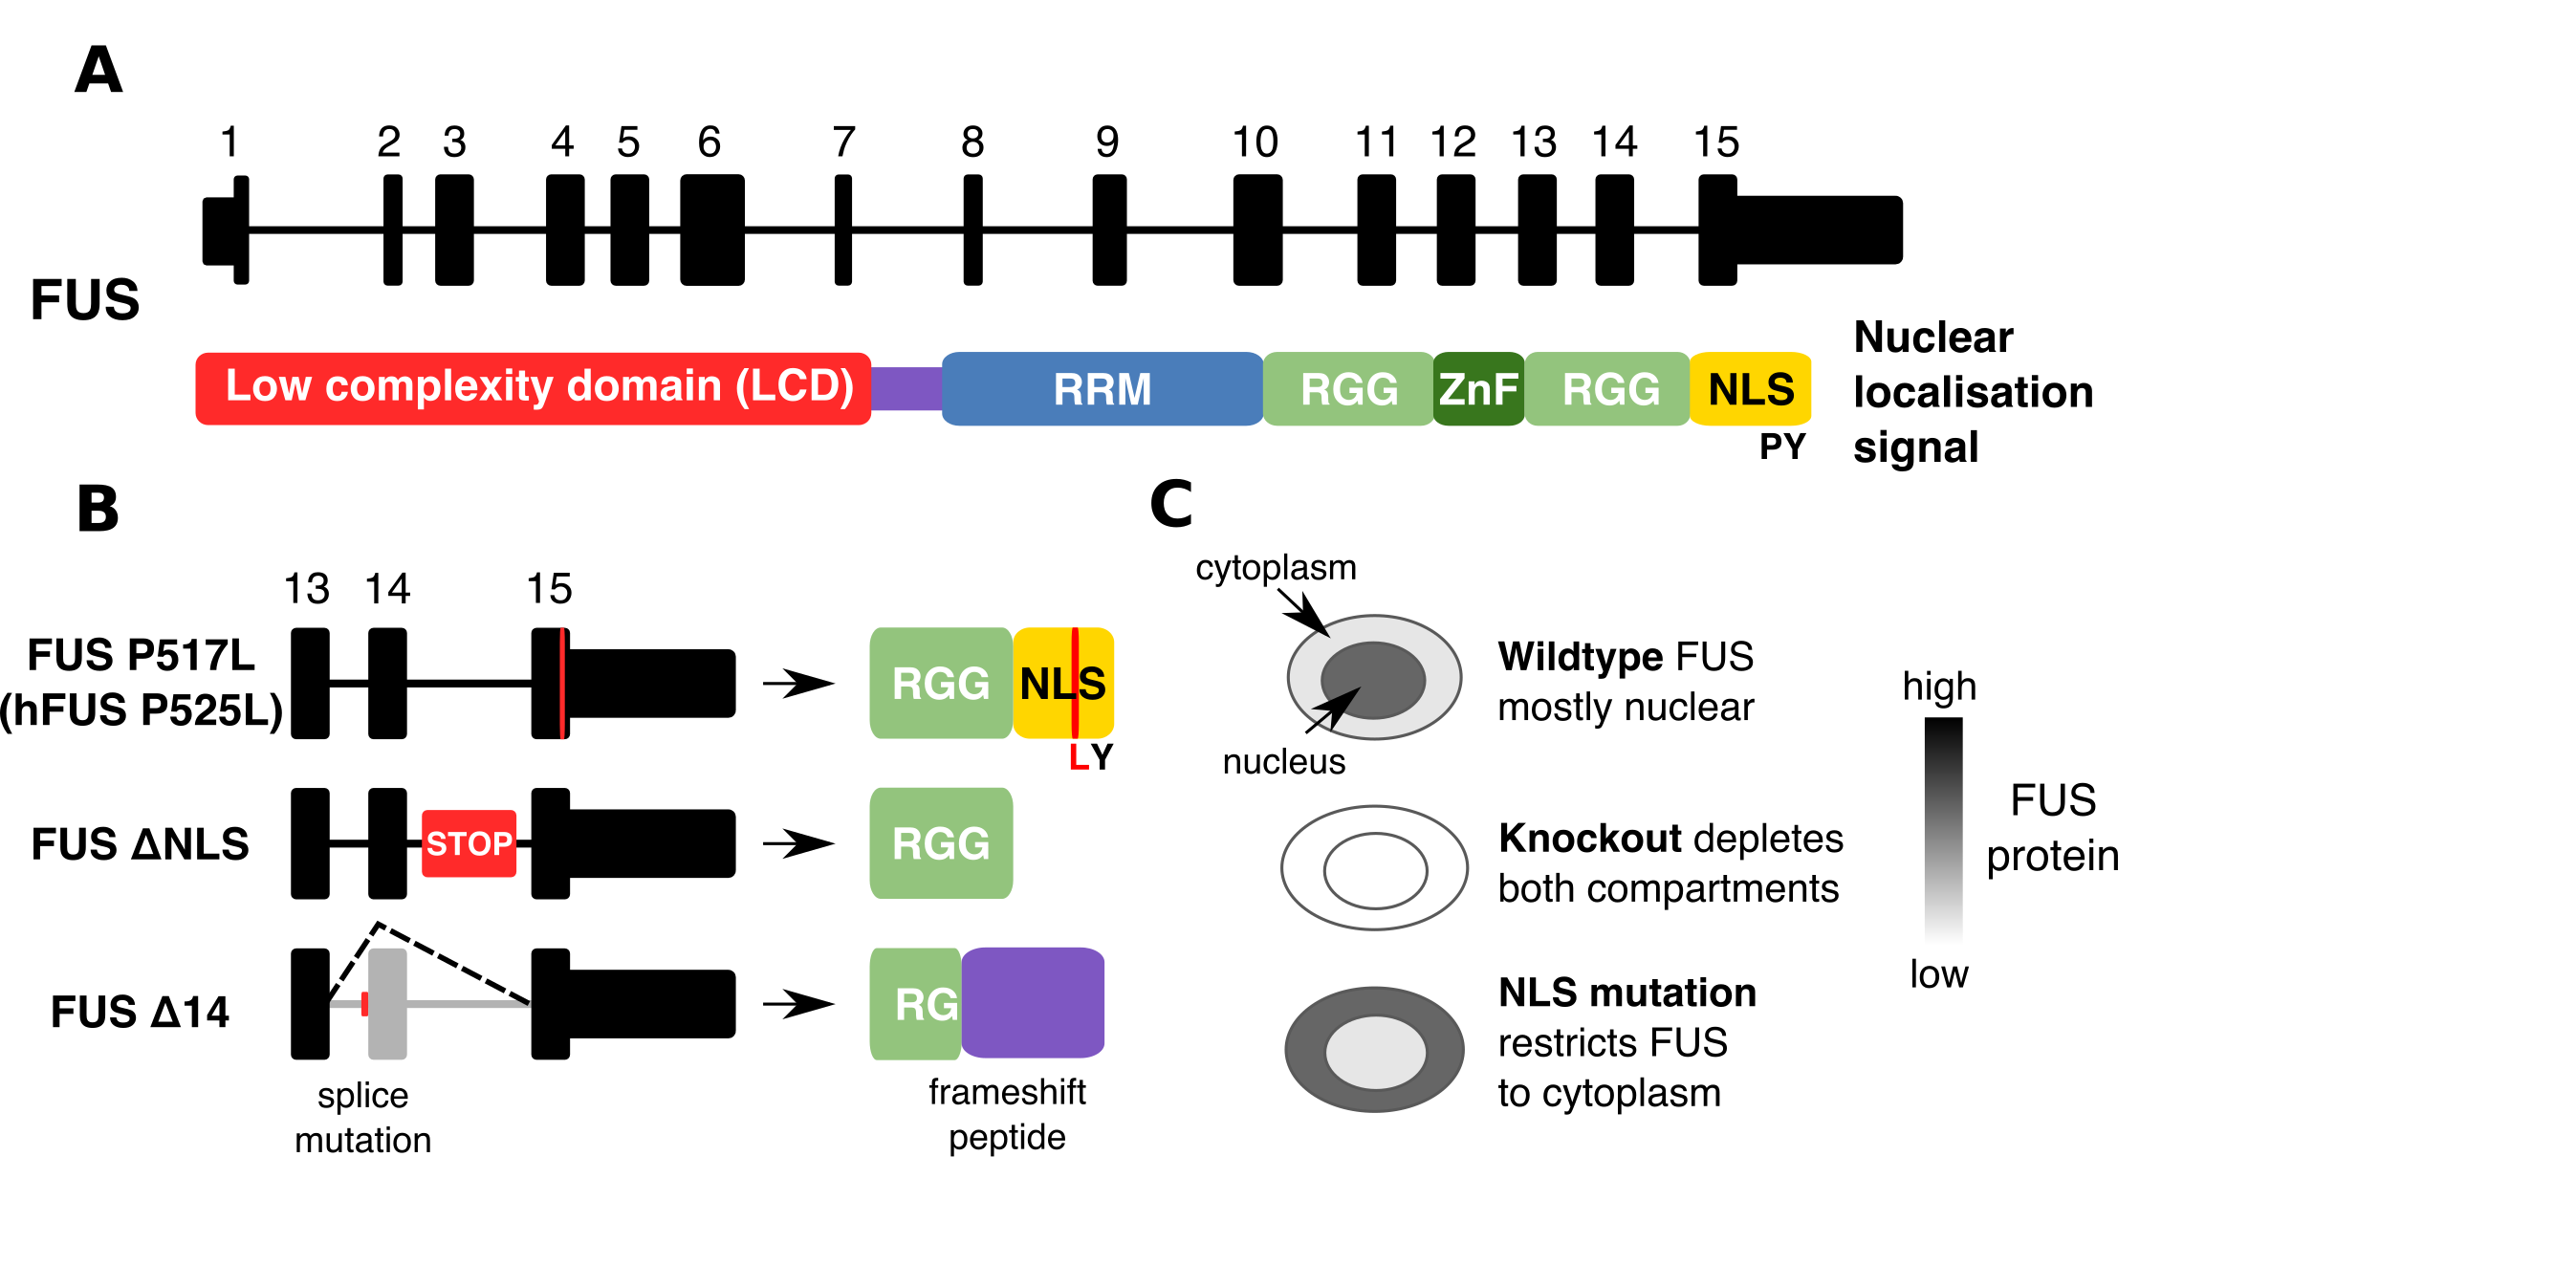
\includegraphics[width=\textwidth]{Figures/06_fus_meta/FUS_structure_mutations.png}
	\caption{\textbf{The structure of the FUS protein and known ALS mutations}}
	A: The \textit{FUS} gene is made up of 15 exons. The FUS protein is comprised of a low complexity domain (LCD), an RNA recognition motif (RRM) domain, two Arginine-Glycine-Glycine (RGG) domains, a zinc finger domain (Znf), a nuclear export signal (NES) and a nuclear localisation signal (NLS). 
	B: The three FUS NLS mutations used in this study. The Bozzoni group knocked in a point mutation to create the FUS P525L line, a missense mutation equivalent to the human ALS P517L mutation.  The Dupuis group created a FUS $\Delta$NLS line where the entire NLS has been removed.  We have used the FUS $\Delta$14 mouse, where a frameshift mutation leads to the skipping of exon 14 and a frameshifting of the remaining NLS sequence.
	C: In wildtype  cells FUS protein is predominantly nuclear but can shuttle to the cytoplasm. When FUS is knocked out or down it will be reduced in both compartments but if the nuclear localisation signal (NLS) is mutated or deleted then FUS will accumulate in the cytoplasm although some will enter the nucleus.
	
	\label{fig:fus_structure}
\end{figure}



\section{Contributions}
% Check with Pietro
RNA sequencing libraries prepared by Dr Nicol Birsa.
Mice handled by Dr Cristian Bodo
RNA extracted for PCR by Dr Nicol Birsa and Matthew Bentham
RT-PCRs performed by David Robaldo and Dr Carmelo Milioto

All bioinformatic analysis and interpretation was performed by myself. The methods section for RT-PCR was written by David Robaldo.


\section{Methods}

\subsection{Data processing}
All RNA sequencing data was processed with our in-house pipeline (see \autoref{chapter:methods}).

\subsection{Differential Expression}
 Each dataset consists of FUS knockout samples, FUS NLS mutation samples and wildtype controls.
In the Bozzoni dataset the controls are shared but in the other two datasets the knockout and mutation samples have their own separate controls for use in two-way comparisons.
Differential gene expression was tested with DESeq2 \citep{Love2014}.
Initially each comparison (wildtype vs knockout or wildtype vs mutation) was run separately for each dataset, creating six individual analyses.
To boost power and create a set of high confidence changes, two joint models were created using either the knockout or mutation samples with their specific controls.
The joint model uses all the samples of the same comparison together in a general linear model with a dataset covariate. 
DESeq2 uses a Bayesian shrinkage strategy when estimating the log2 fold change. Due to high inter-dataset variability this results in very small fold changes being called.
For each gene the $log_2$ fold change is the linear combination of the three individual datasets.
Genes are reported as significantly differentially expressed at a False Discovery Rate threshold of 0.05. 
For plots, gene expression values are  raw counts multiplied by each samples’ size factor generated by DESeq2. 
The points are then normalised to the wildtype samples for each dataset to show the relative change in expression.

To assess the level of overlap between the KO and MUT joint models, two different overlap thresholds were employed.
The first, a more conservative threshold, depends on a gene being significant at FDR < 0.05 in both datasets.
The second, more relaxed threshold, calls a gene as significant if it falls below FDR < 0.05 in one dataset and has an uncorrected p-value < 0.05 in the other.

\subsection{Differential Splicing}
The SGSeq (Goldstein) \citep{Goldstein2016}] package was run on all the samples together to discover and classify all potential splicing events using the default parameters for finding novel splicing. 
Differential splicing for individual comparisons and joint models with a dataset-specific covariate were performed using DEXSeq \cite{Anders2012}.
The same overlap threshold strategies were employed as for differential gene expression.
SGSeq looks for all potential splicing events in each sample and then counts the reads supporting each the inclusion or exclusion of that splicing variant. 
Percentage Spliced In (PSI) values (Katz) \citep{Katz2010-ir} for each splicing variant were calculated by taking the read counts supporting the inclusion event and dividing by the total reads in that event. 
% will I bother doing this?
%For individual splicing events, PSI values were compared between each condition using a one-way ANOVA with post-hoc Tukey test.

\subsection{Gene Ontology}
Gene Ontology enrichment testing was performed with the GProfileR package \citep{Reimand2016}. 
GO and KEGG categories were hand-curated to remove redundant terms and restricted to a minimum overlap of 5 genes per set. 
All P-values  are reported after Bonferroni correction. 

\subsection{iCLIP and functional analyses}

FUS iCLIP data from mouse brain \citep{Rogelj2012} was reprocessed by the iCOUNT iCLIP analysis pipeline (http://icount.biolab.si/). 
I downloaded the set of iFUS iCLIP clusters that passed enrichment against background at FDR < 0.05. 
Only iCLIP clusters with a minimum of two supporting reads were used. 
Untranslated region (UTR) and coding exon (CDS) annotation were taken from GENCODE mouse (comprehensive; mouse v12). Any intron-retention, nonsense mediated decay or "cds end nf" transcripts were removed. 
UTR coordinates were split into 5' and 3' UTR based on whether they overlapped an annotated polyadenylation site or signal (GENCODE mouse v18 poladenylation annotation). 
3'UTRs were extended by 5kb downstream to capture any unannotated sequence.
Introns were defined as any gaps in the transcript model between CDS and UTR coordinates.
Promoter-antisense coordinates were taken by flanking the 5'UTR sequence by 5kb upstream and inverting the strand.
Overlaps between iCLIP peaks and genomic features were created for each set of differentially expressed genes, split into upregulated ($log_2$ fold change > 0 ) or downregulated ($log_2$ fold change < 0). Overlaps were done in a strand-specific manner, with only iCLIP clusters in the same direction being used.
The difference in proportions of upregulated and downregulated genes for each feature were tested with the $\chi^2$ test of equal proportions.

% functional enrichment tests
For the splicing events found in the joint models, three enrichment tests were performed for different genomic features. 
For these tests the coordinates of the entire encompassing intron were used for each splicing variant.
For a null set of splicing events for comparison, a randomly chosen set of 1000 splicing events of each type were used.
Proportions of overlap between splicing events and the null expectation were tested using a $\chi^2$ test of equal proportions.

The coordinates of polyadenylation cleavage sites were downloaded from the PolyA Site Atlas \citep{Gruber2016}. (URL). 
The proportions of  splicing events that overlapped a polyadenylation cleavage site were compared to the null.

The proportion of events of each variant type that overlapped at least one iCLIP peak  were compared to the null expectation.

Per nucleotide PhyloP conservation scores \citep{Pollard2010-fj} comparing mouse (mm10) with 60 other vertebrates was downloaded from UCSC. 
The median PhyloP score calculated for each splicing variant and compared.

\subsection{RT-PCR}
Primers were designed using Primer3 \citep{Koressaar2007} and in silico PCR (UCSC). 
For both human and mouse FUS, the forward primer was designed for exon 6 and the reverse primer designed to span the spliced exon 8/9 junction to preferentially amplify spliced FUS mRNA. 
An additional third primer was designed to amplify a section of either intron 6 or intron 7.

Cells were obtained from mouse brains and/or cultured mouse embryonic fibroblasts resuspended in trizol. 
RNA was extracted using miRNeasy Mini Kit (Qiagen) following the manufacturer's instructions % what kit did Nicol use?
cDNA was obtained from extracted RNA using SuperScript IV Reverse Transcriptase kit (Invitrogen). 
Briefly, a mix was made of RNA template (500ng for mouse brain; 100ng for cultured cells (cycloheximide treatment), 10 mM dNTP, 50 mM oligo d(T)20, 50 mM random hexamer followed by 5 min of incubation at 65$\degree$C and 1 min in ice. Mix was then complemented with 5X SuperScript IV Reverse Transcriptase buffer, 100 nM DTT, RNase OUT and SuperScript IV Reverse Transcriptase buffer followed by incubation at 23$\degree$C, 55$\degree$C and 80$\degree$C, 10 min each. 

RT-PCR was carried out using 10X AccuPrime Taq DNA polymerase mastermix system (Invitrogen). 
Each PCR reaction mix contained 5 ng of gDNA, 10 mM of forward and reverse primers. cDNA was amplified with the following conditions:
Intron 6 retention: One cycle of 5 min at 95$\degree$C, followed by 30 cycles of 30 sec at 95$\degree$C, 30 sec at 56$\degree$C, and 30 sec at 68$\degree$C, and finishing with 5 min incubation at 68$\degree$C.
Intron 7 retention: One cycle of 5 min at 95$\degree$C, followed by 30 cycles of 30 sec at 95$\degree$C, 30 sec at 61$\degree$C, and 30 sec at 68$\degree$C, and finishing with 5 min incubation at 68$\degree$C.
Srsf7 NMD positive control: One cycle of 5 min at 95 $\degree$C, followed by 35 cycles of 30 sec at 95 $\degree$C, 30 sec at 58 $\degree$C, and 15 sec at 68 $\degree$C, and finishing with 5 min incubation at 68 $\degree$C.
Amplified products were finally obtained using Agilent 4200 TapeStation System following the manufacturer's instructions. Results were analysed on TapeStation analysis software.
Intron retention events are plotted  as the percentage of integrated area of the retained band.



\begin{table}[h!]
	%\begin{centerline}
	\centering
	\begin{tabular}{rcl}
		\textbf{Target} & \textbf{Direction} & \textbf{Sequence}\\
		\hline \\[-0.3cm]
		mFUS exon 6  & F &  GTTATGGCAATCAGGACCAGAG\\
		mFUS intron 6 & R & TTGGCTCCCAAGTTCTCACA\\
		mFUS intron 7 & F &  GGAGAAACTGGATGGATGCAC\\
		mFUS exon 8/9 & R &  CCTGTTCAGAATCATGACGAGA\\[0.2cm]
		hFUS exon 6 & F & TCCTCCATGAGTAGTGGTGGT \\
		hFUS intron 6 & R & GTTCAGGCTCCCAAGTTCTC\\
		hFUS intron 7 & F & TTCTCTCGGGTGAGAGAACC\\
		hFUS exon 8/9 & R & GTCTGAATTATCCTGTTCGGAGTC\\[0.2cm]
		mSRSF7 & F &  CGACGAAGAAGAAGCAGGTTTC\\
		mSRSF7& R & TCTGGCCTCTTATGCTGATCAC\\
	\end{tabular}
	%\end{centerline}
	\caption{List of primers used in RT-PCR. mFUS: mouse \textit{FUS}; hFUS: human \textit{FUS}}
	\label{tab:fus_primers}
\end{table}

\subsection{Cycloheximide treatment and fractionation}
Mouse embryonic fibroblasts were treated with 100ug/ml cycloheximide for 6 hours before RNA was extracted with Trizol (Thermo Fisher) and RT-PCR performed as before. 
As a positive control, primers targeting the NMD-sensitive exon 4 of \textit{Srsf7} were taken from \citep{Edwards2016}.

\clearpage


\section{Results}

\subsection{ Comparing three RNA-seq datasets of FUS knockout and FUS mutation}

% Discuss 3 datasets, pros and cons of each
% differences in sequencing, prediction
For this study, three datasets of FUS knockout (KO) and FUS nuclear localisation signal mutation (FUS MUT) were used.

% Bozzoni
The lab of Irene Bozzoni at the University of Rome generated RNA-seq data from purified motor neurons cultured from mouse induced pluripotent stem cells. 
Their knockout uses a gene trap in exon 12 first used in \citep{Hicks2000}, which leads to a partial reduction of FUS protein levels.
Their NLS mutation is a point mutation affecting the penultimate amino acid of the NLS which in humans is the very aggressive ALS mutation P525L, which translates in mice to P517L.  
All mice are homozygous for their transgenes. 
The two conditions share a single set of controls, which are motoneurons derived from wildtype stem cells.
The read depth and length is moderately high but the sample number is the lowest of the three datasets  (n=3 for each condition).
The Bozzoni dataset was published as \citep{Capauto2018}.

%Dupuis
The lab of Luc Dupuis from INSERM, Strasbourg generated RNA-seq data from mouse embryonic brain (day E18.5). 
Their knockout construct uses a gene trap in intron 1 (generated by themselves) as this creates a more effective knockout than the intron 12 gene trap.  
Their NLS mutation introduces a stop codon after exon 14, terminating transcription upstream of the NLS sequence. 
All mice are homozygous for their transgenes. 
The two conditions have their own separate wildtype littermate controls. 
The depth and read length of the RNA-seq libraries is shorter than the other two datasets but this is compensated for by being polyA+ enriched, which will mean a greater proportion of sequencing reads aligning to coding exons.  
This will be useful for assessing differential expression but I predict the dataset will not be particularly useful for differential splicing due to the low read dept and read length.
The Dupuis dataset was published as \citep{Scekic-zahirovic2016}.

% Fratta
The third dataset was created for this study using mouse embryonic spinal cords (embryonic day E18.5). The knockout construct is the same as the Dupuis dataset so should be a robust knockout of FUS. 
The NLS mutation is the $\Delta$14 mutation discussed in \autoref{chapter:fus_mouse}, where a splice site mutation prevents the inclusion of exon 14, causing a downstream frameshift and ablation of the entire NLS. 
The wildtype littermate controls are separate for each condition. 
For both conditions, heterozygous mice with only one mutant allele were also generated and sequenced.
The RNA-seq data produced is of the highest quality of the three datasets, with 150bp reads and high depth. 
This will be useful in quantifying differential splicing, although as it is total RNA rather than polyA+ enriched there will be a lot of pre-mRNA present.


\begin{longtable}[]{@{}llllll@{}}
	\begin{minipage}[t]{0.14\columnwidth}\raggedright\strut
		{\textbf{Dataset}}\strut
	\end{minipage} & \begin{minipage}[t]{0.14\columnwidth}\raggedright\strut
		{\textbf{Tissue}}\strut
	\end{minipage} & \begin{minipage}[t]{0.12\columnwidth}\raggedright\strut
		{\textbf{Controls}}\strut
	\end{minipage} & \begin{minipage}[t]{0.10\columnwidth}\raggedright\strut
		{\textbf{Age}}\strut
	\end{minipage} & \begin{minipage}[t]{0.14\columnwidth}\raggedright\strut
		{\textbf{Knockout (KO)}}\strut
	\end{minipage} & \begin{minipage}[t]{0.14\columnwidth}\raggedright\strut
		{\textbf{Mutation (MUT)}}\strut
	\end{minipage}\tabularnewline\toprule \\[-0.3cm] 
	\begin{minipage}[t]{0.16\columnwidth}\raggedright\strut
		{\textbf{Bozzoni}}
		{\footnotesize\citep{Capauto2018}}\strut
	\end{minipage} & \begin{minipage}[t]{0.14\columnwidth}\raggedright\strut
		{Motor neurons}
		{cultured from iPSCs}\strut
	\end{minipage} & \begin{minipage}[t]{0.12\columnwidth}\raggedright\strut
		{Shared}\strut
	\end{minipage} & \begin{minipage}[t]{0.10\columnwidth}\raggedright\strut
		{-}\strut
	\end{minipage} & \begin{minipage}[t]{0.16\columnwidth}\raggedright\strut
		{Gene trap in exon 12}	
		{ \footnotesize\citep{Hicks2000} }\strut
	\end{minipage} & \begin{minipage}[t]{0.16\columnwidth}\raggedright\strut
		{P517L knock-in,}
		{corresponding to human P525L}
		{\footnotesize\citep{Chio2009} }\strut
	\end{minipage}\tabularnewline \\
	\begin{minipage}[t]{0.16\columnwidth}\raggedright\strut
		{\textbf{Dupuis}}
		{\footnotesize\citep{Scekic-zahirovic2016}}\strut
	\end{minipage} & \begin{minipage}[t]{0.14\columnwidth}\raggedright\strut
		{Whole brain}\strut
	\end{minipage} & \begin{minipage}[t]{0.12\columnwidth}\raggedright\strut
		{Separate}\strut
	\end{minipage} & \begin{minipage}[t]{0.10\columnwidth}\raggedright\strut
		{E18.5}\strut
	\end{minipage} & \begin{minipage}[t]{0.16\columnwidth}\raggedright\strut
		{Gene trap in intron 1}\strut
	\end{minipage} & \begin{minipage}[t]{0.16\columnwidth}\raggedright\strut
		{Stop codon after exon 14 ($\Delta$NLS)}\strut
	\end{minipage}\tabularnewline \\
	\begin{minipage}[t]{0.16\columnwidth}\raggedright\strut
		{\textbf{Fratta}}\strut
	\end{minipage} & \begin{minipage}[t]{0.14\columnwidth}\raggedright\strut
		{Spinal cord}\strut
	\end{minipage} & \begin{minipage}[t]{0.12\columnwidth}\raggedright\strut
		{Separate}\strut
	\end{minipage} & \begin{minipage}[t]{0.10\columnwidth}\raggedright\strut
		{E18.5}\strut
	\end{minipage} & \begin{minipage}[t]{0.16\columnwidth}\raggedright\strut
		{Gene trap in intron 1}\strut
	\end{minipage} & \begin{minipage}[t]{0.16\columnwidth}\raggedright\strut
		{$\Delta$ exon 14 }
		{\footnotesize\citep{Devoy2017}}  \strut
	\end{minipage}\tabularnewline
	\caption{The three FUS mouse datasets}
	\label{tab:fus_datasets}
\end{longtable}

% SEQUENCING STATS

\begin{longtable}[]{@{}llllll@{}}
	\begin{minipage}[t]{0.14\columnwidth}\raggedright\strut
		{\textbf{Dataset}}\strut
	\end{minipage} & \begin{minipage}[t]{0.14\columnwidth}\raggedright\strut
		{\textbf{Replicates per condition}}\strut
	\end{minipage} & \begin{minipage}[t]{0.14\columnwidth}\raggedright\strut
		{\textbf{Library type}}\strut
	\end{minipage} & \begin{minipage}[t]{0.14\columnwidth}\raggedright\strut
		{\textbf{Mapped reads (millions)}}\strut
	\end{minipage} & \begin{minipage}[t]{0.14\columnwidth}\raggedright\strut
		{\textbf{Read type}}\strut
	\end{minipage} & \begin{minipage}[t]{0.14\columnwidth}\raggedright\strut
		{\textbf{SRA accession}}\strut
	\end{minipage}\tabularnewline\toprule \\[-0.3cm]
	\begin{minipage}[t]{0.14\columnwidth}\raggedright\strut
		{\textbf{Bozzoni} }\strut
	\end{minipage} & \begin{minipage}[t]{0.14\columnwidth}\raggedright\strut
		{3}\strut
	\end{minipage} & \begin{minipage}[t]{0.14\columnwidth}\raggedright\strut
		{Total RNA}\strut
	\end{minipage} & \begin{minipage}[t]{0.14\columnwidth}\raggedright\strut
		{34-52}\strut
	\end{minipage} & \begin{minipage}[t]{0.14\columnwidth}\raggedright\strut
		{2 x 100bp}\strut
	\end{minipage} & \begin{minipage}[t]{0.14\columnwidth}\raggedright\strut
		{SRP111475}\strut
	\end{minipage}\tabularnewline \\
	\begin{minipage}[t]{0.14\columnwidth}\raggedright\strut
		{\textbf{Dupuis}}\strut
	\end{minipage} & \begin{minipage}[t]{0.14\columnwidth}\raggedright\strut
		{4-5}\strut
	\end{minipage} & \begin{minipage}[t]{0.14\columnwidth}\raggedright\strut
		{mRNA}\strut
	\end{minipage} & \begin{minipage}[t]{0.14\columnwidth}\raggedright\strut
		{15-25}\strut
	\end{minipage} & \begin{minipage}[t]{0.14\columnwidth}\raggedright\strut
		{1 x 50bp}\strut
	\end{minipage} & \begin{minipage}[t]{0.14\columnwidth}\raggedright\strut
		{SRP070906 }\strut
	\end{minipage}\tabularnewline \\
	\begin{minipage}[t]{0.14\columnwidth}\raggedright\strut
		{\textbf{Fratta} }\strut
	\end{minipage} & \begin{minipage}[t]{0.14\columnwidth}\raggedright\strut
		{4}\strut
	\end{minipage} & \begin{minipage}[t]{0.14\columnwidth}\raggedright\strut
		{Total RNA}\strut
	\end{minipage} & \begin{minipage}[t]{0.14\columnwidth}\raggedright\strut
		{52-65}\strut
	\end{minipage} & \begin{minipage}[t]{0.14\columnwidth}\raggedright\strut
		{2 x 150bp}\strut
	\end{minipage} & \begin{minipage}[t]{0.14\columnwidth}\raggedright\strut
		{-}\strut
	\end{minipage}\tabularnewline
	\caption{RNA-seq statistics of the three datasets}
	\label{tab:fus_sequencing}
\end{longtable}


\subsection{Modelling differential expression jointly boosts power and demonstrates significant overlap between FUS knockout and FUS NLS mutation}

% Explain individual analyses
Differential expression compares the abundances of each gene's RNA between two conditions. 
As most RNA-sequencing datasets comprise small numbers of samples, the number of genes found to be significantly changed between conditions highly depends on the degree of difference between conditions, the number of samples per condition, and the read depth covering each gene. The more sequencing reads that cover a gene, the more precise the measure of the true variance can be.
Most software packages attempt to get round these hurdles by borrowing information across all genes to shrink the variance between samples of the same condition. 
When I analyse each dataset individually, comparing KO and MUT to their respective controls in each dataset, the Dupuis dataset had the largest number of differentially expressed genes in both conditions (FDR < 0.05), an order of magnitude more than Bozzoni or Fratta. 
This is probably due to a larger sample size and the fact that their data is polyA+ enriched, which will potentially reduce the between-sample variation allowing for more precise measures of between-condition differences. 
It is also possible that however they prepared the tissues and extracted the RNA resulted in less variability between samples than the Bozzoni and Fratta datasets.
Despite the differences in numbers, in all three datasets the knockout condition produces more differentially expressed genes than NLS mutation, suggesting a stronger effect on FUS function.


% Combining datasets in a joint model increases power, shrinks effect sizes
I chose to combine the three datasets together in a joint analysis for the knockout and NLS mutation samples and their respective controls. 
This increases the sample size of each condition from 3-5 to 11-12 which should markedly improve the estimation of per-gene variation. 
DESeq2 uses a general linear model framework so I simply added a dataset-specific covariate. 
This strategy will reward genes where the direction of change is the same between all three datasets and punish genes where the datasets differ in direction. 
The two comparisons are nominally independent from each other as only the Bozzoni wildtype samples are shared.
Modelling all the data together allows the three independent studies of FUS function to contribute to a high-confidence set of expression changes. At a false discovery rate threshold of 0.05 the joint models for the knockout comparison (KO) and the NLS mutation comparison (MUT) find 2136 and 754 significantly altered genes respectively. 
When comparing the genes found by the joint analysis to the individual analyses there is only a moderate overlap. 
Of the 2916 genes found in the Dupuis KO comparison, only 1007 of those genes are present in the joint analysis.
This suggests that a large number of genes called as significant in the Dupuis dataset cannot be replicated in the other two, despite being the same condition and all being embryonic neuronal tissue.

\begin{figure}[h!]
	\centering
	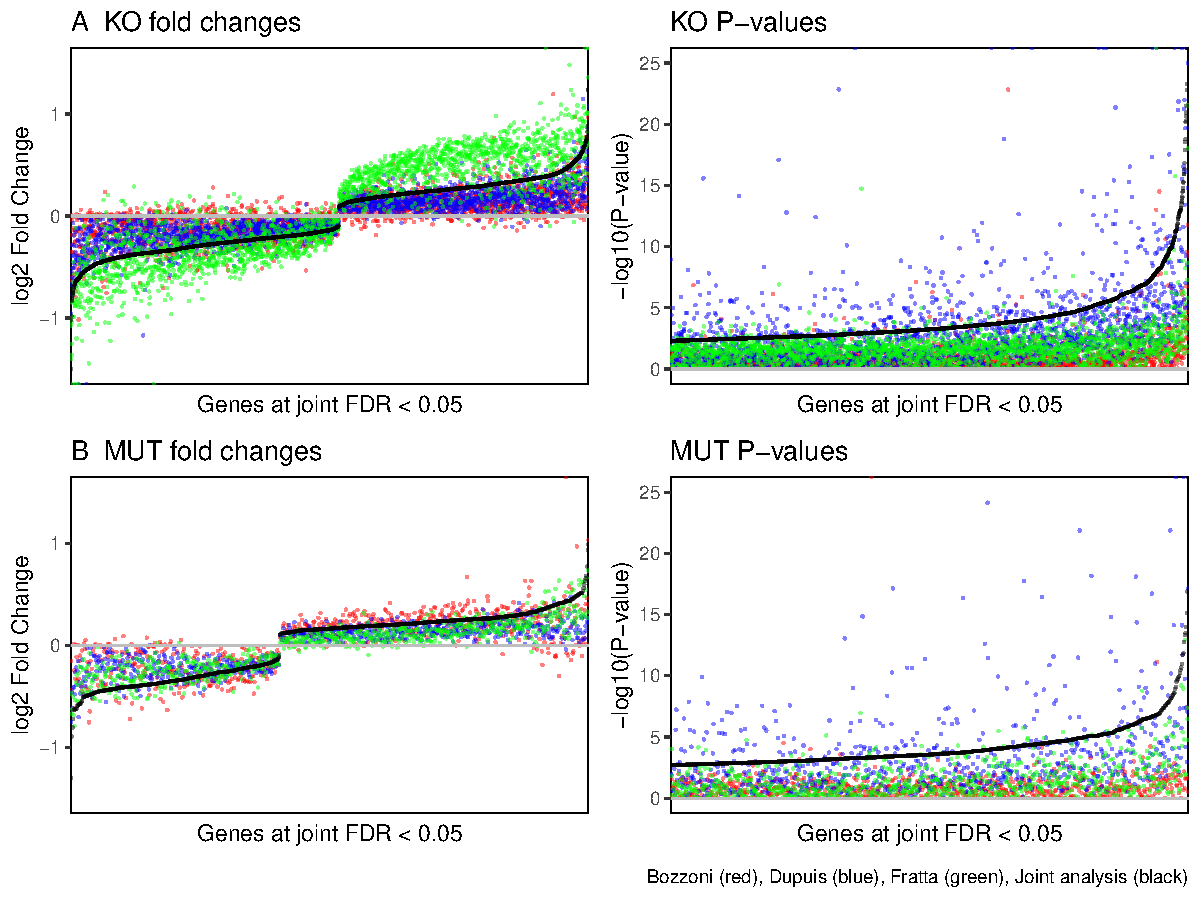
\includegraphics[width=\textwidth]{Figures/06_fus_meta/fitted_vs_individual_p_lfc.pdf}
	\caption{\textbf{Joint differential expression increases power and adjusts effect sizes}}
	A: Plotting the $log_2$ fold changes (left) and P-values (right) for the 2136 KO genes and 754 MUT genes found at FDR < 0.05 in the two joint analyses. Values found in the individual analyses, Bozzoni (red), Dupuis(blue) and Fratta (green) are compared to the value produced by the joint analysis (black).
	B: As before but for the MUT analyses.
	\label{fig:value_comparison}
\end{figure}

For each gene the resulting joint $log_2$ fold change and P-value is an estimated combination of the three datasets.
I compared the values found by the individual analyses with the joint models \ref{fig:value_comparison}.
For the KO models, the Fratta KO dataset has inflated $log_2$ fold change values compared to Bozzoni and Dupuis. 
The fitted $log_2$ fold change is a compromise between the estimated fold changes of all three datasets. 
When inspecting the distribution of P-values, the Dupuis KO dataset has a large excess of low P-values due to the lower within-condition variance.
Therefore the joint modelling strategy increases the number of genes and harmonises three different datasets together into a set of high confidence differentially expressed genes.

% Explain strict and relaxed overlap

\begin{figure}[h!]
	\centering
	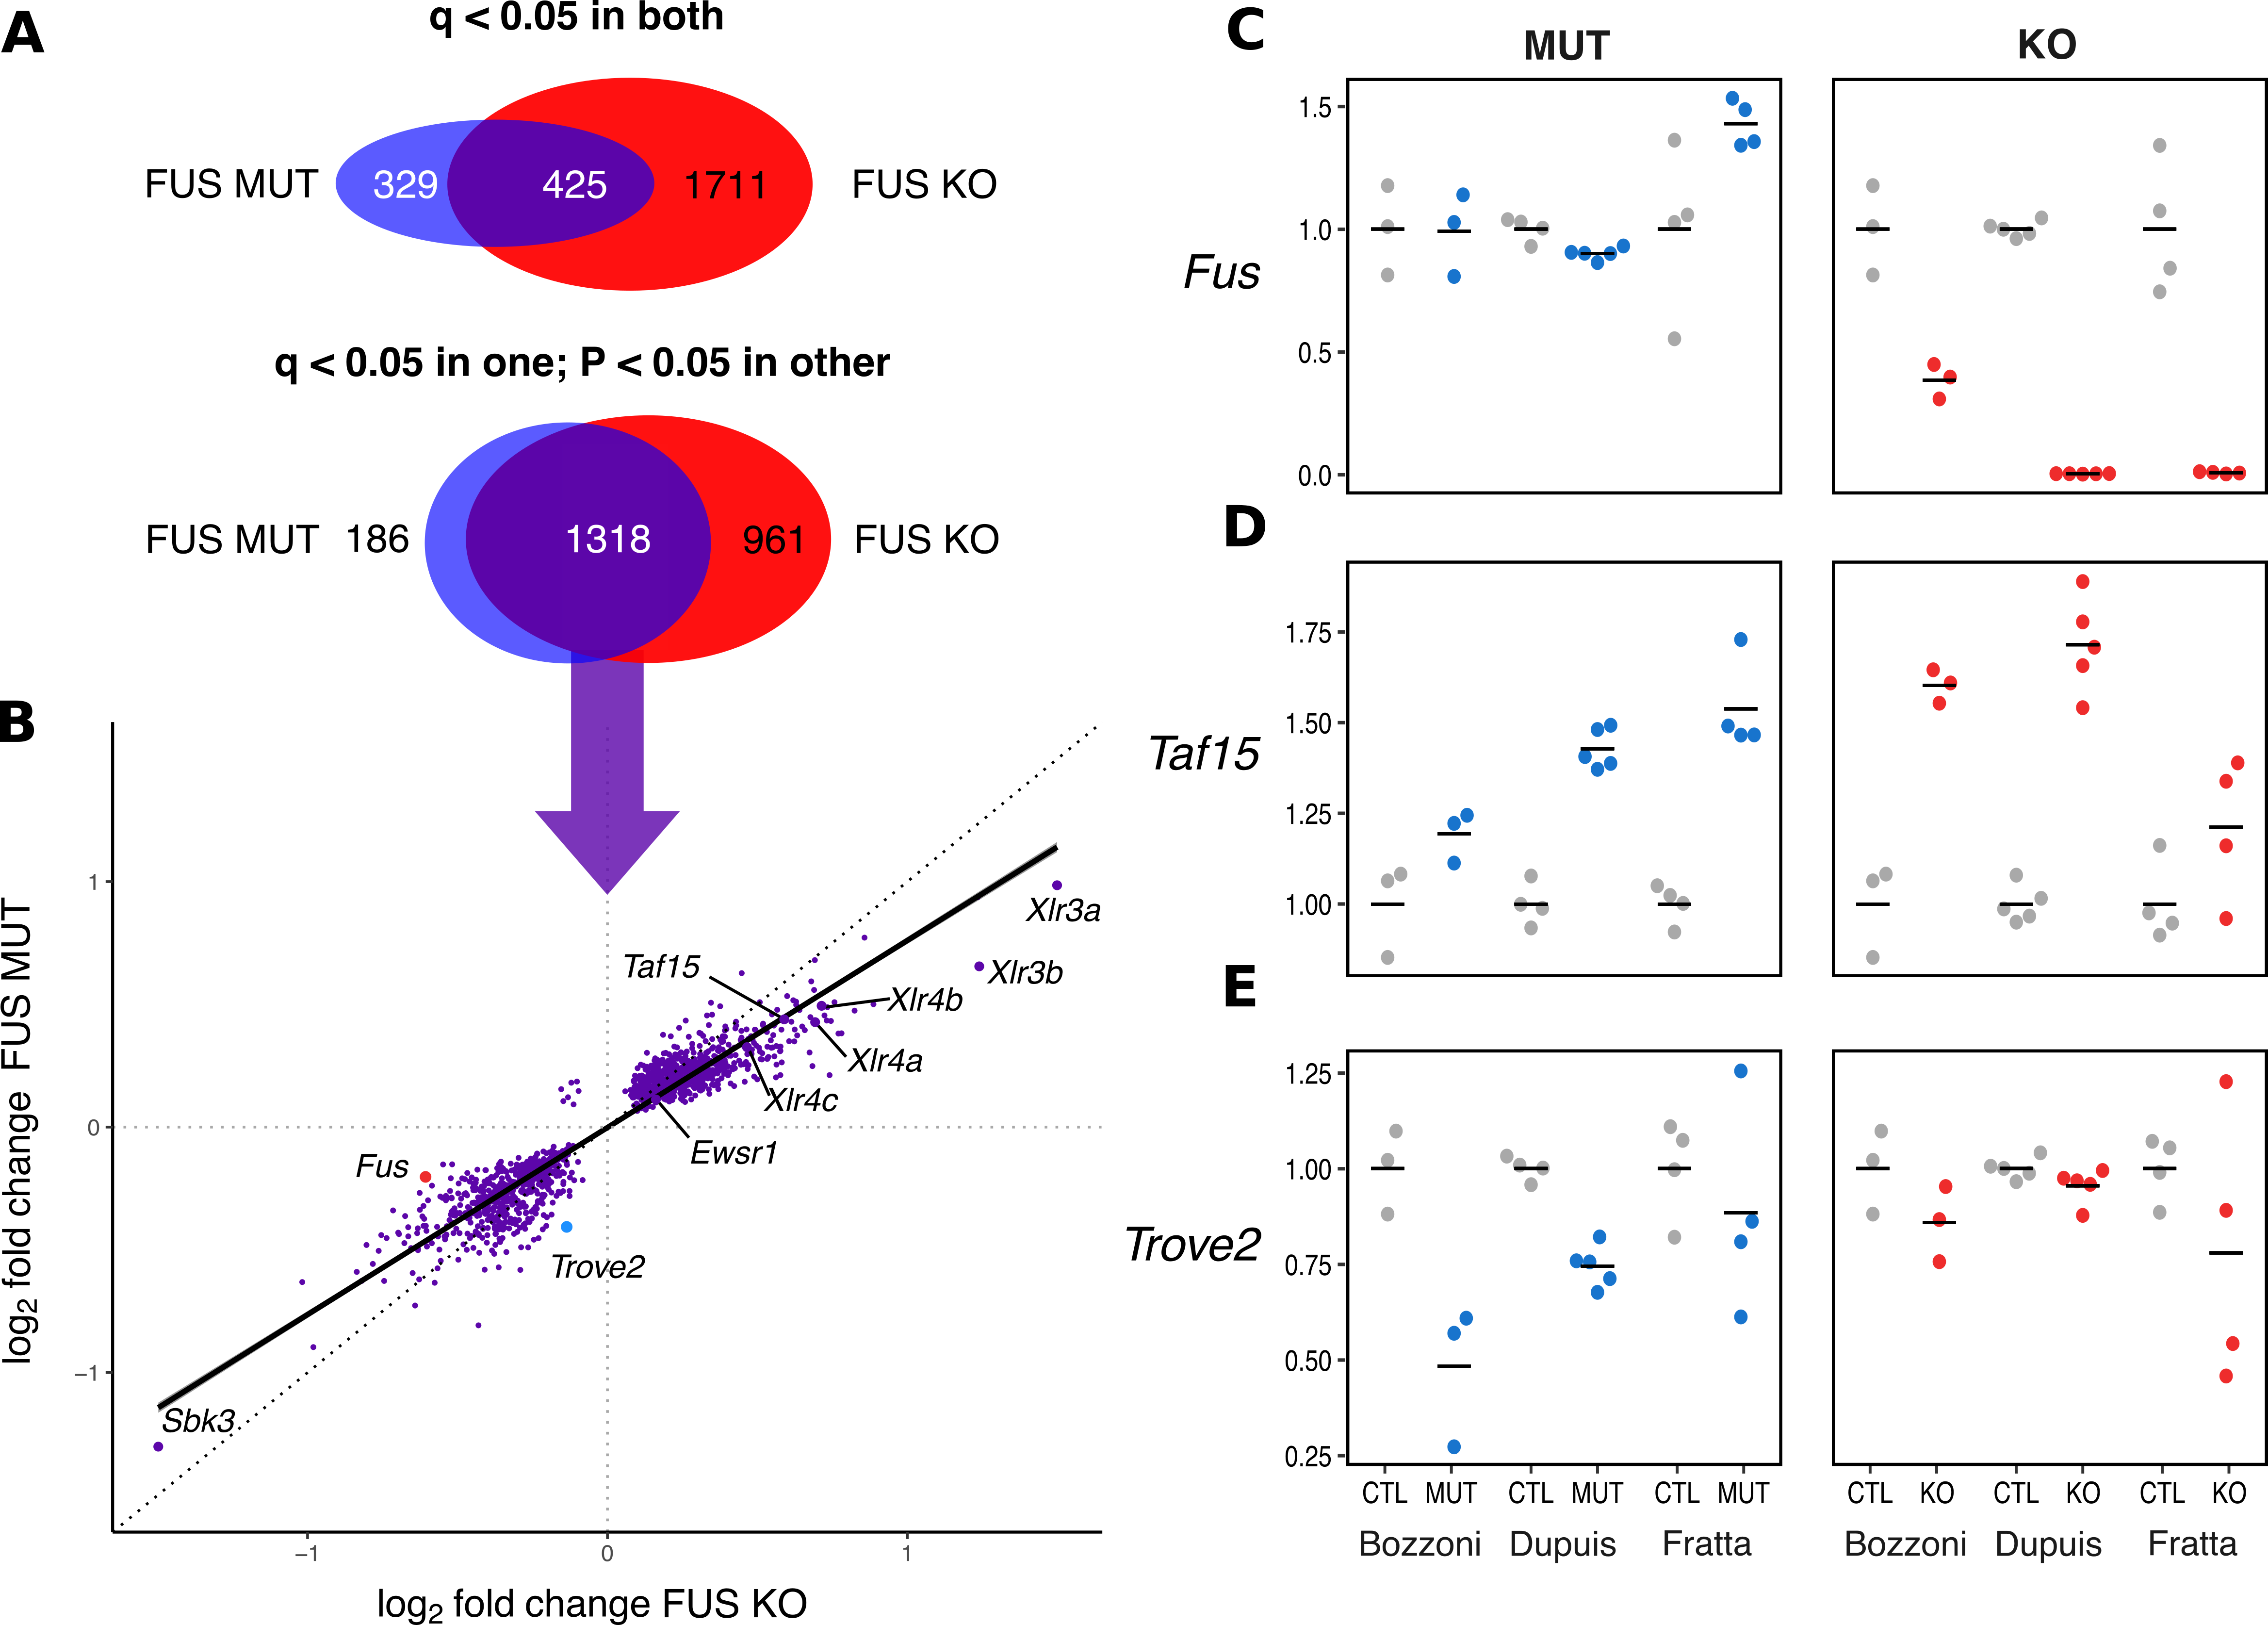
\includegraphics[width=\textwidth]{Figures/06_fus_meta/expression_multi.png}
	\caption{\textbf{Overlapping the joint differential expression models shows that FUS mutations affect gene expression in generally the same direction}}
	A: Venn diagrams show the overlap between the FUS KO and FUS MUT joint differential expression models with a strict FDR cut-off (upper) and a more relaxed P-value cut-off. 
	B: Plotting the fitted $log_2$ fold-change values for each of the 1318 overlapping genes in KO and MUT shows a bias towards weaker changes in MUT compared to KO.
	C, D,E: Normalised read counts in each dataset for \textit{Fus}, \textit{Taf15} and \textit{Trove2}. Samples are plotted relative to the mean expression in controls (CTL).
	\label{fig:fus_expression_multipanel}
\end{figure}

The two joint models provide a set of genes where we can be confident of a shared signal between all three datasets.  
I wanted to look for evidence of a shared gene expression signal between the KO model and the MUT model.
If there truly is a cytoplasmic gain of FUS function on gene expression then I would expect to see a set of genes specific to NLS mutation or a set of overlapping genes that change in opposing directions.
Taking a conservative threshold for overlap, where a gene must be significant at FDR < 0.05 in both models, leads to a moderate overlap of 425 shared genes between KO and MUT ( Figure \ref{fig:fus_expression_multipanel} A), with 329 mutation-specific genes and 1711 knockout specific genes.
However if we employ a relaxed overlap criteria to FDR < 0.05 in one model and an uncorrected P < 0.05 in the other then we can see a substantial overlap of 1318 genes, where the majority of genes are now shared between both conditions.
This relaxed overlap reduces the number of genes I classify as mutation-specific to 186, and knockout specific to 961.

% comparing directions in the overlapping genes
Comparing the log$_2$ fold changes of the 1318 overlapping genes between FUS KO and FUS MUT shows that only 7 genes are altered in opposing directions (0.5\%).
Fitting a linear model between the fold changes of the two datasets shows that the effect of FUS MUT on gene expression is 76\% that of FUS KO.  ($\beta$ = 0.76; P < 1e-16 F-test; $R^2$ = 0.90).

This suggests that while FUS KO and FUS MUT affect the same genes in the same directions, the strength of change is greater in FUS KO than FUS MUT. 
This could be explained by nuclear FUS depletion driving the expression changes.
This relationship is not an artefact of the relaxed overlap criteria as fitting the model on just the 425 strictly overlapping genes results in $\beta = 0.8; P < 1e-16$. % R^2?
Nuclear depletion will be stronger in the knockout than in the NLS mutations as mutant FUS is still transported to nucleus albeit at a much reduced level \citep{Devoy2017, Scekic-zahirovic2016}.

% individual hits
Visualising single genes in all the datasets demonstrates the power of the joint models.
It also clearly shows the higher within-condition variance in the Fratta dataset compared to the Dupuis dataset.
\textit{Fus} itself is unchanged in the FUS MUT joint model  but strongly downregulated in FUS KO (Figure \ref{fig:fus_expression_multipanel}C), leading to its classification as KO specific.
The Bozzoni knockout transgene is indeed weak, with a reduction of \textit{Fus} RNA to only 40\% of wildtype, compared to near 100\% knockout in the other two datasets.
The other members of the FET family of RNA-binding proteins,  \textit{Taf15} and \textit{Ewsr1} have been shown to reciprocally interact with FUS at protein-protein  \citep{Kapeli2016} and protein-RNA \citep{Lagier-Tourenne2012}.
\textit{Taf15} is strongly upregulated in both MUT and KO (Figure \ref{fig:fus_expression_multipanel}D), as is \textit{Ewsr1}.  \textit{Taf15} upregulation was validated by the Dupuis group  \citep{Scekic-zahirovic2016} % other citations too.
The \textit{Trove2} gene encoding the 60 kDa SS-A/Ro ribonucleoprotein,  is downregulated in MUT only and unchanged in KO (Figure \ref{fig:fus_expression_multipanel}E).

\textit{Sbk3}, SH3 Domain Binding Kinase Family Member 3, has the strongest negative change in both conditions. % write some guff about SBK3

The X-linked lymphocyte receptor genes, \textit{Xlr3a, Xlr3b, Xlr4a} and \textit{Xlr4b} are all strongly upregulated in both conditions but more so in KO than MUT. 

These genes form a cluster of paralogous genes on the X chromosome and are paternally imprinted in mice \cite{Raefski2005} and have been shown to alter dendritic spine growth when overxpressed \citep{Cubelos2010}. 
Although these changes have been observed in another FUS knockout mouse model \citep{Kino2015}, I was concerned that these changes were drive by an imbalance of sexes between conditions as embryonic mice are not typically sexed.
I was able to sex the samples \textit{in silico} using the read counts aligning to chrY-specific genes (see Appendices). 
Although there is an imbalance between sexes it is clearly not driving the large upregulation of \textit{Xlr} genes . 
The upregulation of \textit{Xlr3a} is strongest within the all-male Bozzoni dataset (Figure \ref{fig:fus_xlr_expression}A) and can also be seen in the mixed-sex Dupuis and Fratta datasets. 
These genes appear to be mouse specific but they raise interesting questions about the role of FUS on gene regulation.

\begin{figure}[h!]
	\centering
	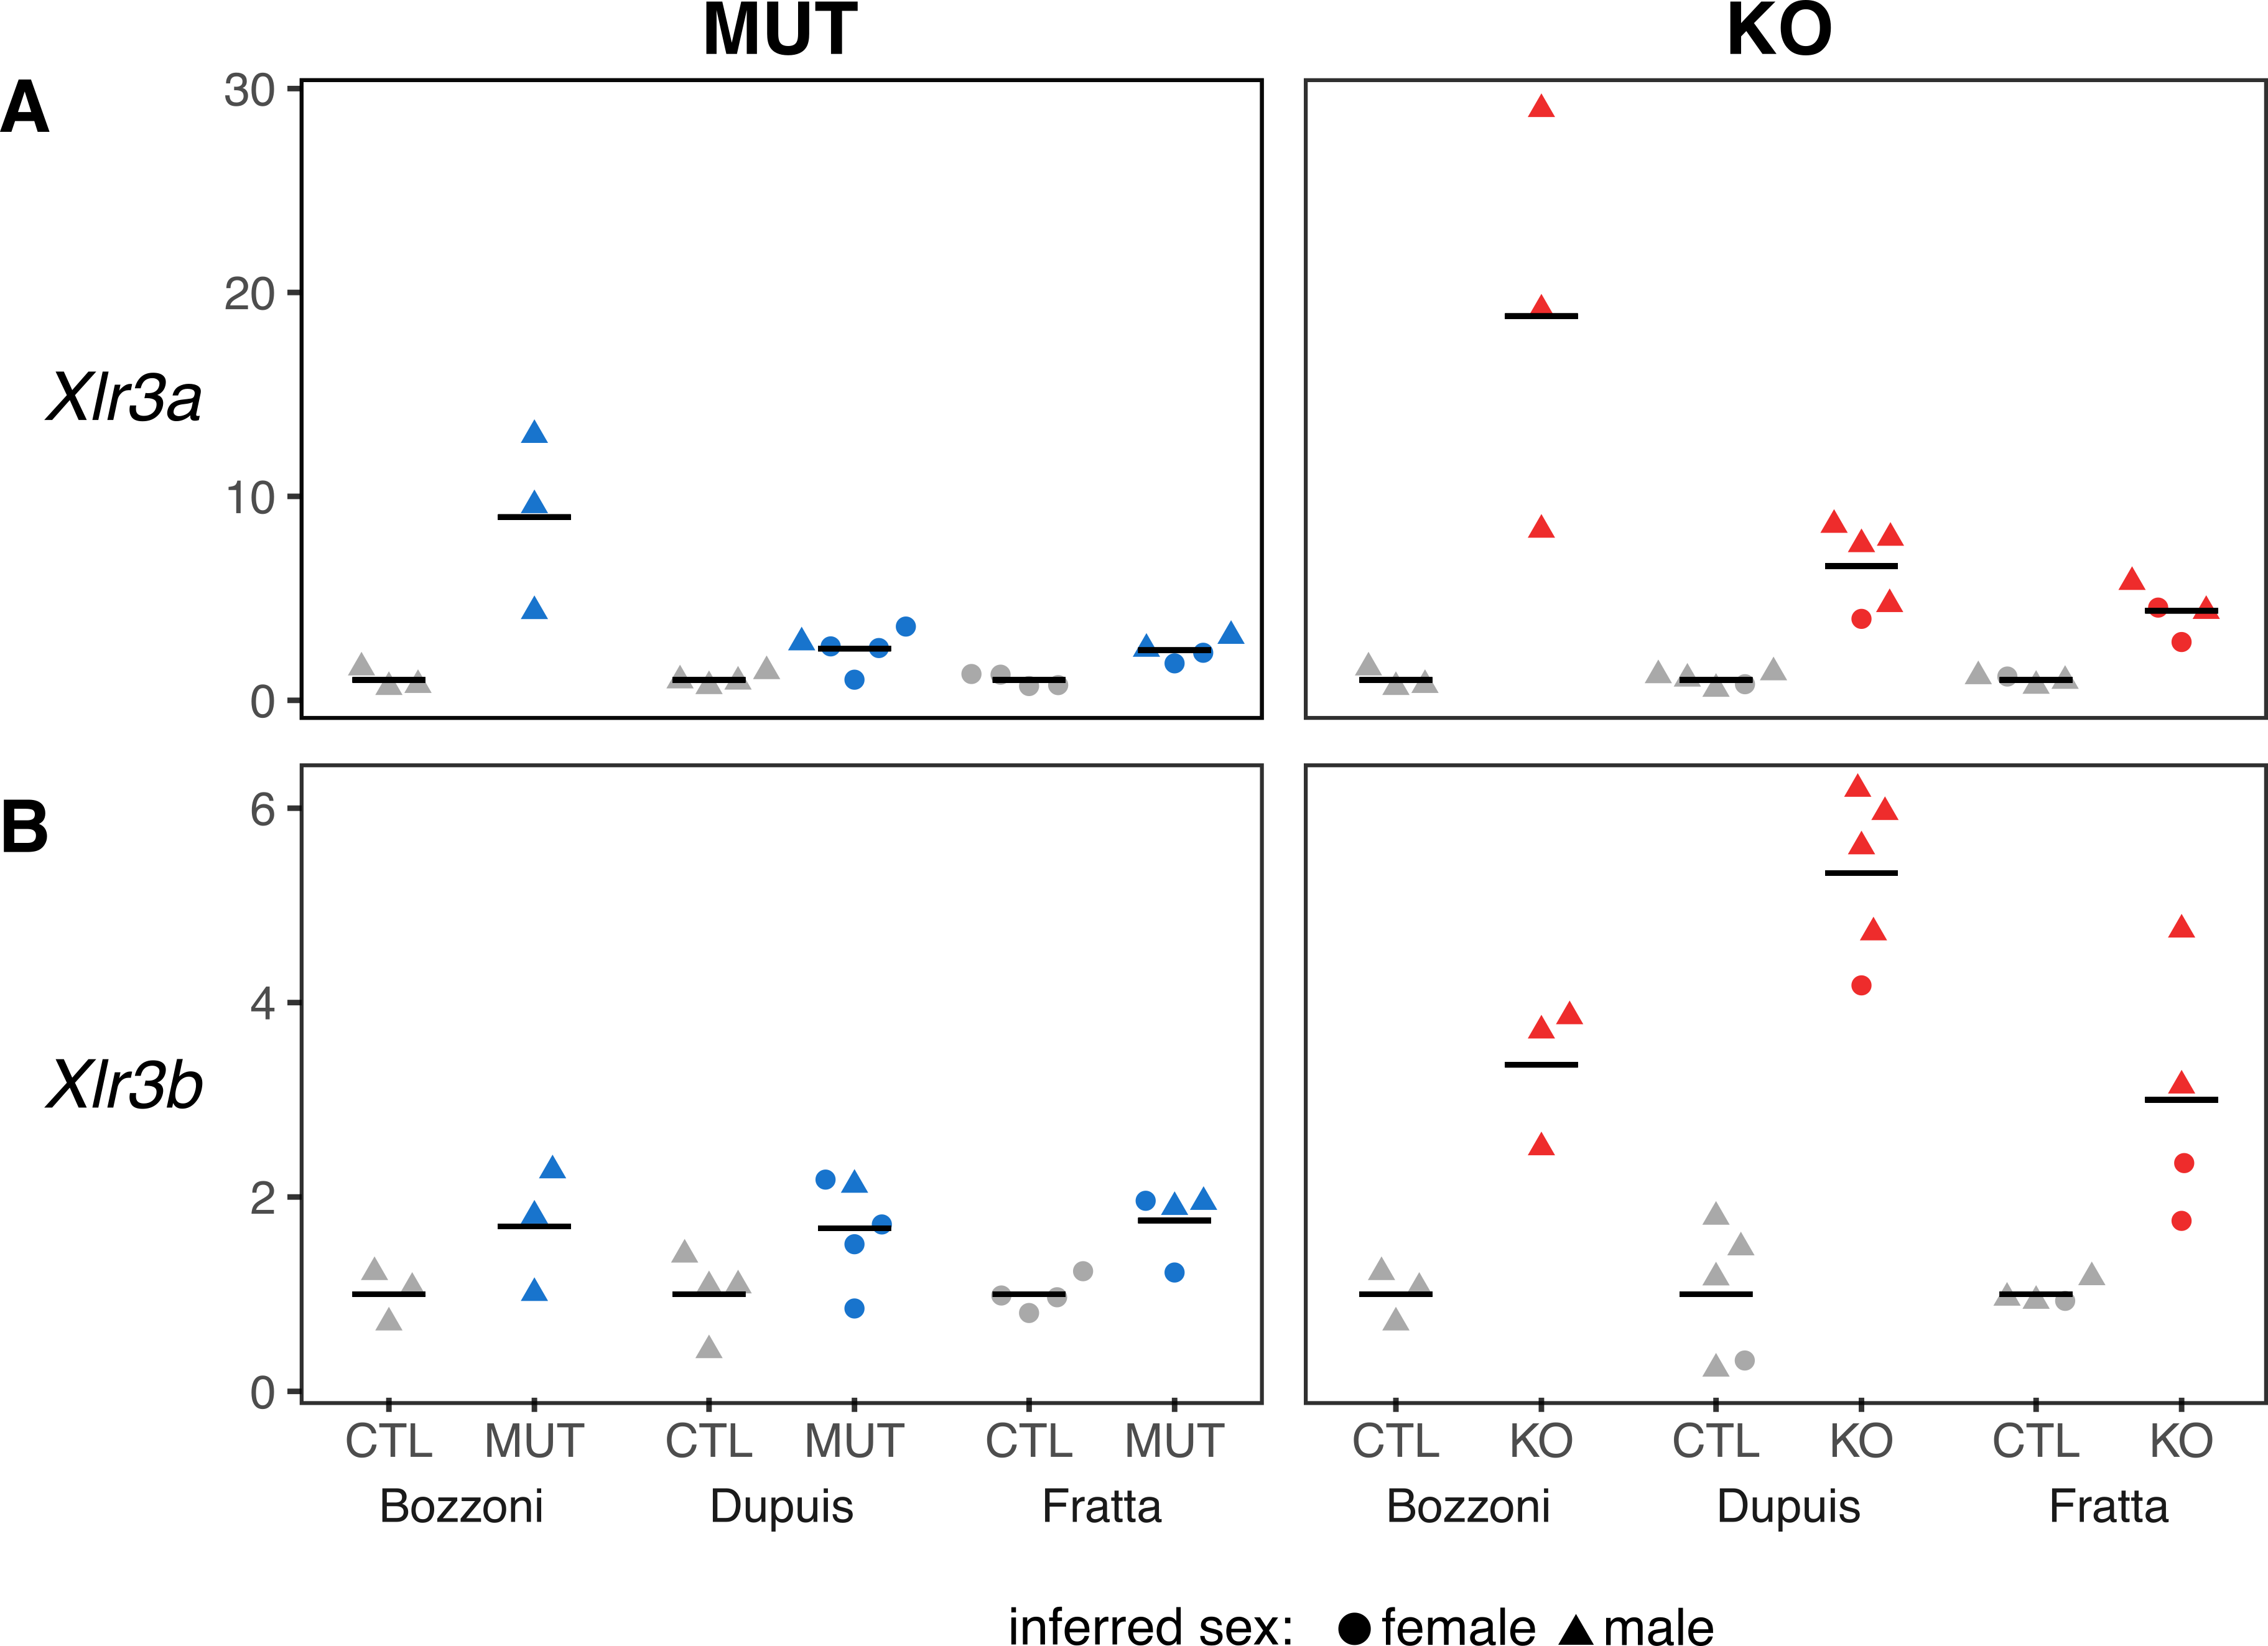
\includegraphics[width=10cm]{Figures/06_fus_meta/xlr_sex_expression.png}
	\caption{\textbf{Xlr genes are strongly upregulated in both FUS KO and FUS MUT} }	
    Normalised read counts in each dataset, plotted relative to the mean of each dataset and condition-specific control group for Xlr3a (A) and Xlr3b (B). 
	\label{fig:fus_xlr_expression}
\end{figure}


%Comparing the log2 fold changes (LFC) between KO and MUT with linear regression demonstrates that the overlapping genes are changed on average 76\% in MUT of the strength in KO. ( lfc_MUT = 0.76 . lfc_KO - 0.0017; P < 1e-16; F-test).

% opposing 7 genes
%Only 7 genes are changed in the opposite direction (0.5%). 3/7 have FUS iCLIP peaks overlapping
%Prickle2 is a synaptic gene, large number of iCLIP peaks in first 250kb intron - long gene!
%Dcaf7 has a 7 read iCLIP peak in the first intron (short intron)
%Cds2 has 2 peaks (7 and 1) in the 3'UTR


\subsection{Synaptic and RNA-binding genes are a common gene expression response to FUS nuclear depletion}

\begin{figure}[h!]
	\centering
	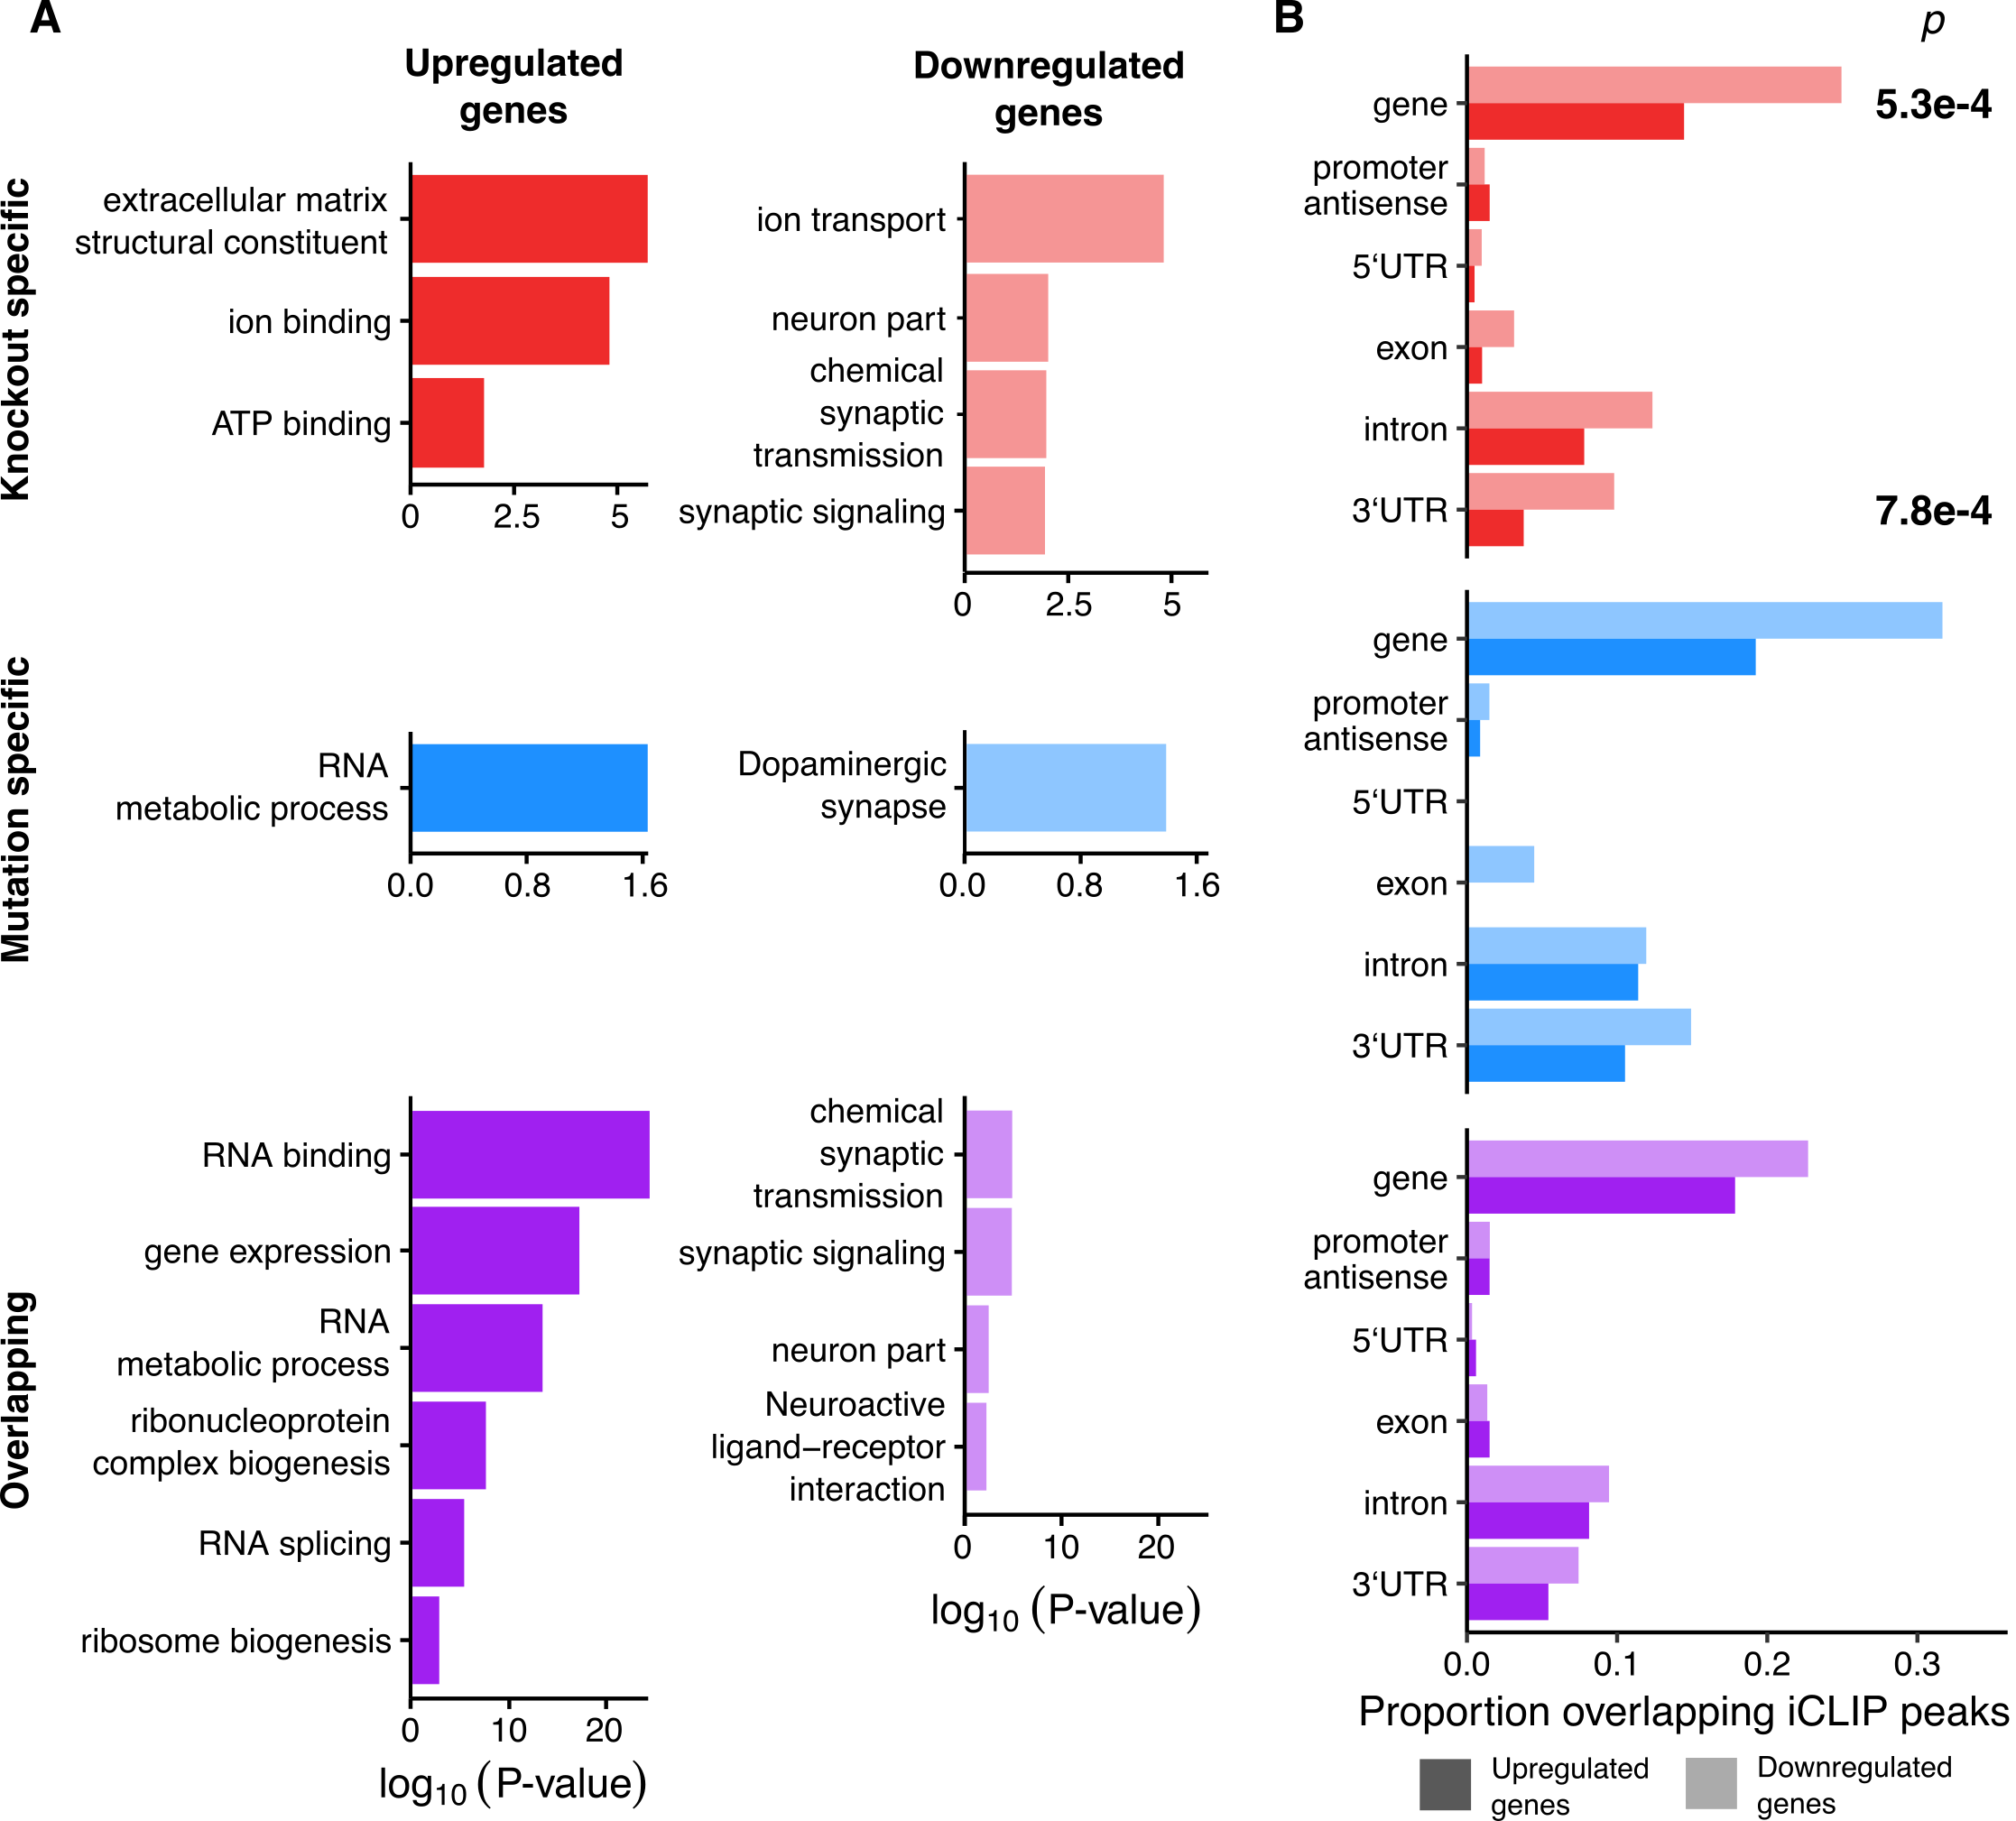
\includegraphics[width=\textwidth]{Figures/06_fus_meta/expression_curated_go_terms.png}
	\caption{\textbf{Overlapping genes are enriched in neuronal and RNA terms} }	
	A: Enriched Gene Ontology terms in the three groups of genes, split by direction.
	B: Proportions of each set of genes that have any iCLIP peaks within the entire gene or in any particular gene feature, split by direction. 
	P values are from $\chi^2$ test of equal proportions. P values presented are those below the Bonferroni corrected threshold of 0.05 / 18 = 0.0028. 
	\label{fig:fus_expression_go}
\end{figure}


Gene ontology (GO) terms enriched in the overlapping genes were strongly direction specific, with upregulated genes enriched in terms involving RNA binding, splicing and metabolism whereas downregulated genes were enriched in synaptic and neuronal terms \ref{fig:fus_expression_go}.
Knockout- and mutation-specific genes were less clearly enriched in specific functions. 
Knockout specific genes were involved in extracellular membrane functions, ion channels and amino acid transport whereas the mutant specific genes showed an enrichment in Dopaminergic synapses and metabolism.


% TABLE OF GENE EXPRESSION NUMBERS
\begingroup
\renewcommand{\arraystretch}{1.5}
\begin{table}[h!]
	%\begin{centerline}
		\begin{tabular}{|r|ccc|ccc|}
			\hline
			& Bozzoni & Dupuis & Fratta & Bozzoni & Dupuis & Fratta\\[-0.3cm]
			& MUT & MUT & MUT & KO & KO & KO\\
			\hline
			Individual hits                & 19 & 1552 & 88 & 100 & 2916 & 151 \\
			Overlapping joint model & 5 & 368 & 57 & 51 & 1007 & 114 \\
			Unique to dataset          & 14 & 1184 & 31 & 49 & 1909 & 37 \\
			\hline
			\textbf{Joint model}       & \multicolumn{3}{c|}{754} & \multicolumn{3}{c|}{2136} \\
			\hline
			Overlap (strict)              & \multicolumn{2}{c}{329} & \multicolumn{2}{|c|}{\textbf{425}} & \multicolumn{2}{c|}{1711} \\
			Overlap (relaxed)           & \multicolumn{2}{c}{186} & \multicolumn{2}{|c|}{\textbf{1318} } & \multicolumn{2}{c|}{961} \\
			\hline
		\end{tabular}
	%\end{centerline}
	\caption{Results from separate and joint differential expression analysis}
	\label{tab:expression_results}
\end{table}
\endgroup


\subsection{ Overlapping genes are bound by FUS in introns and 3'UTRs}

Individual nucleotide resolution crosslinking and immunopreciation (iCLIP) is an experimental technique for identifying the RNA targets of RNA-binding proteins. 
Using iCLIP and other RNA-protein interaction technqieus, FUS has been shown to preferentially bind within introns and 3' untranslated regions (3'UTR) of many mRNAs rather than exons \citep{Lagier-Tourenne2012-wa, Rogelj2012, Ishigaki2012, Masuda2015a}. 
FUS binding at the 3'UTR has been shown to influence polyadenylation of certain genes \citep{Masuda2015a} but may also have a role in directing mRNA localisation or competing with microRNAs, which predominantly bind 3'UTR sequences to trigger degradation.
A small number of genes have been reported to have FUS binding upstream of the promoter antisense to the gene which was reported to correlate with upregulation of the gene upon FUS knockdown \citep{Ishigaki2012}.
I used the coordinates of FUS binding sites enriched relative to a background control in a published FUS iCLIP dataset from mouse brain \citep{Rogelj2012} to investigate a relationship between specific FUS binding and the direction of gene expression in the different gene sets.


The iCLIP binding profiles of the three sets of genes are similar with introns and 3'UTR sequences being most commonly bound (Figure \ref{fig:fus_expression_go}B), despite introns being far longer.
Comparing the proportion of upregulated and downregulated genes that change only in FUS KO, there is an enrichment in iCLIP peaks in downregulated genes (P =5.3e-4, $\chi^2$ test of equal propotions ), an enrichment driven primarily by 3'UTR binding (P = 7.8e-4). 
This direction preference is not seen in the mutation specific (FUS MUT) or overlapping gene sets.
Promoter-antisense binding is found in a small number of genes at a constant proportion between gene set and direction.
% caveat - iCLIP is from predominantly nuclear WT FUS, mutation-specific genes may be bound differently (more exon).


%% SPLICING

\subsection{FUS modulates the inclusion of a set of highly conserved RNA-binding protein introns}

I then used the same joint modelling approach to assess evidence of differing effects between FUS knockout and NLS mutation on alternative splicing.
For the individual analyses I ran SGSeq\citep{Goldstein2016} to discover and quantify all possible alternative splicing isoforms, both novel and annotated. 
The read counts supporting each splicing variant were used to test for differential usage of each splicing variant between conditions for either MUT or KO.
For the joint analyses, I ran SGSeq on all the samples simultaneously and then fit a generalised linear model for each splicing variant for the KO and MUT conditions separately with their specific controls using a dataset-specific covariate in DEXSeq \citep{Anders2012}..
Table \ref{tab:splicing_results} summarises the numbers of splicing events found at FDR < 0.05.
Here the weakness of the Dupuis samples for capturing splicing is revealed, presumably due to the short single-end sequencing reads. 
The joint models perform better here for boosting power as for MUT and KO respectively 93 and 890 events are found to be significantly altered, more than the sum of the individual analyses.
There is also a very good concordance between the individual analyses and the joint model, with the exception of the Bozzoni mutant samples (only 7 out of 31).

Comparing the joint FUS knockout and NLS mutation splicing models, the two overlap at both a strict and relaxed significance threshold.
With the relaxed overlap criteria there are almost no NLS mutation specific splicing events at al;, as only 16 remain (Figure \ref{fig:fus_splicing_multi}.
There are 501 knockout specific splicing events and 405 that overlap between the two conditions.
Manual inspection of the 16 mutant specific genes gave little confidence of a mutation-specific effect on splicing, as all but one splicing event appeared convincingly in all 3 datasets.
The single event that did appear to be real was an intron retention event in \textit{FUS}, far upstream of the mutated NLS region.

% types of splicing event - how many are annotated?
Comparing the different types of splicing event shows a similar distribution between KO specific and overlapping splicing events, dominated by complex splicing events.
These splicing events are combinations of multiple types, such as a cassette exon accompanied by a retained intron and multiple alternative 3' and 5' splice sites, all overlapping within the same region. When using tools like SGSeq that can pick up novel splicing events it can be expected that the majority of events are indeed complex, a phenomenon also seen with the MAJIQ splicing tool \citep{Vaquero-Garcia2016}.
An example of a complex event is in \textit{Ybx1}, which comprises a cassette exon within a retained intron.
The second largest category of event are retained introns.
An example of this can be seen in the FUS interacting RNA binding protein \textit{Ewsr1}, where a normally retained intron is less retained in both FUS knockout and NLS mutation.
The third largest category are the "classical" cassette exons, which can either be skipped or included. 
An example is an annotated cassette exon in the neuronal gene \textit{Nrxn3}, which is included more in FUS knockout and NLS mutation, but is not expressed in the Bozzoni motoneuron samples.
RNA-seq traces of each event are in the appendices.
% expand on this or not?
Alternate 5' and 3' splice sites can be found in all three sets of genes, with alternate 5' sites appearing at twice the rate of alternate 3' splice sites. FUS is known to interact with the U1 snRNP \citep{Yu2015a,Yu2015b}., and so knockdown or NLS mutation of FUS could feasibly impair U1 snRNP binding and disrupt 5' splice site recognition.


\begin{figure}[h!]
	\centering
	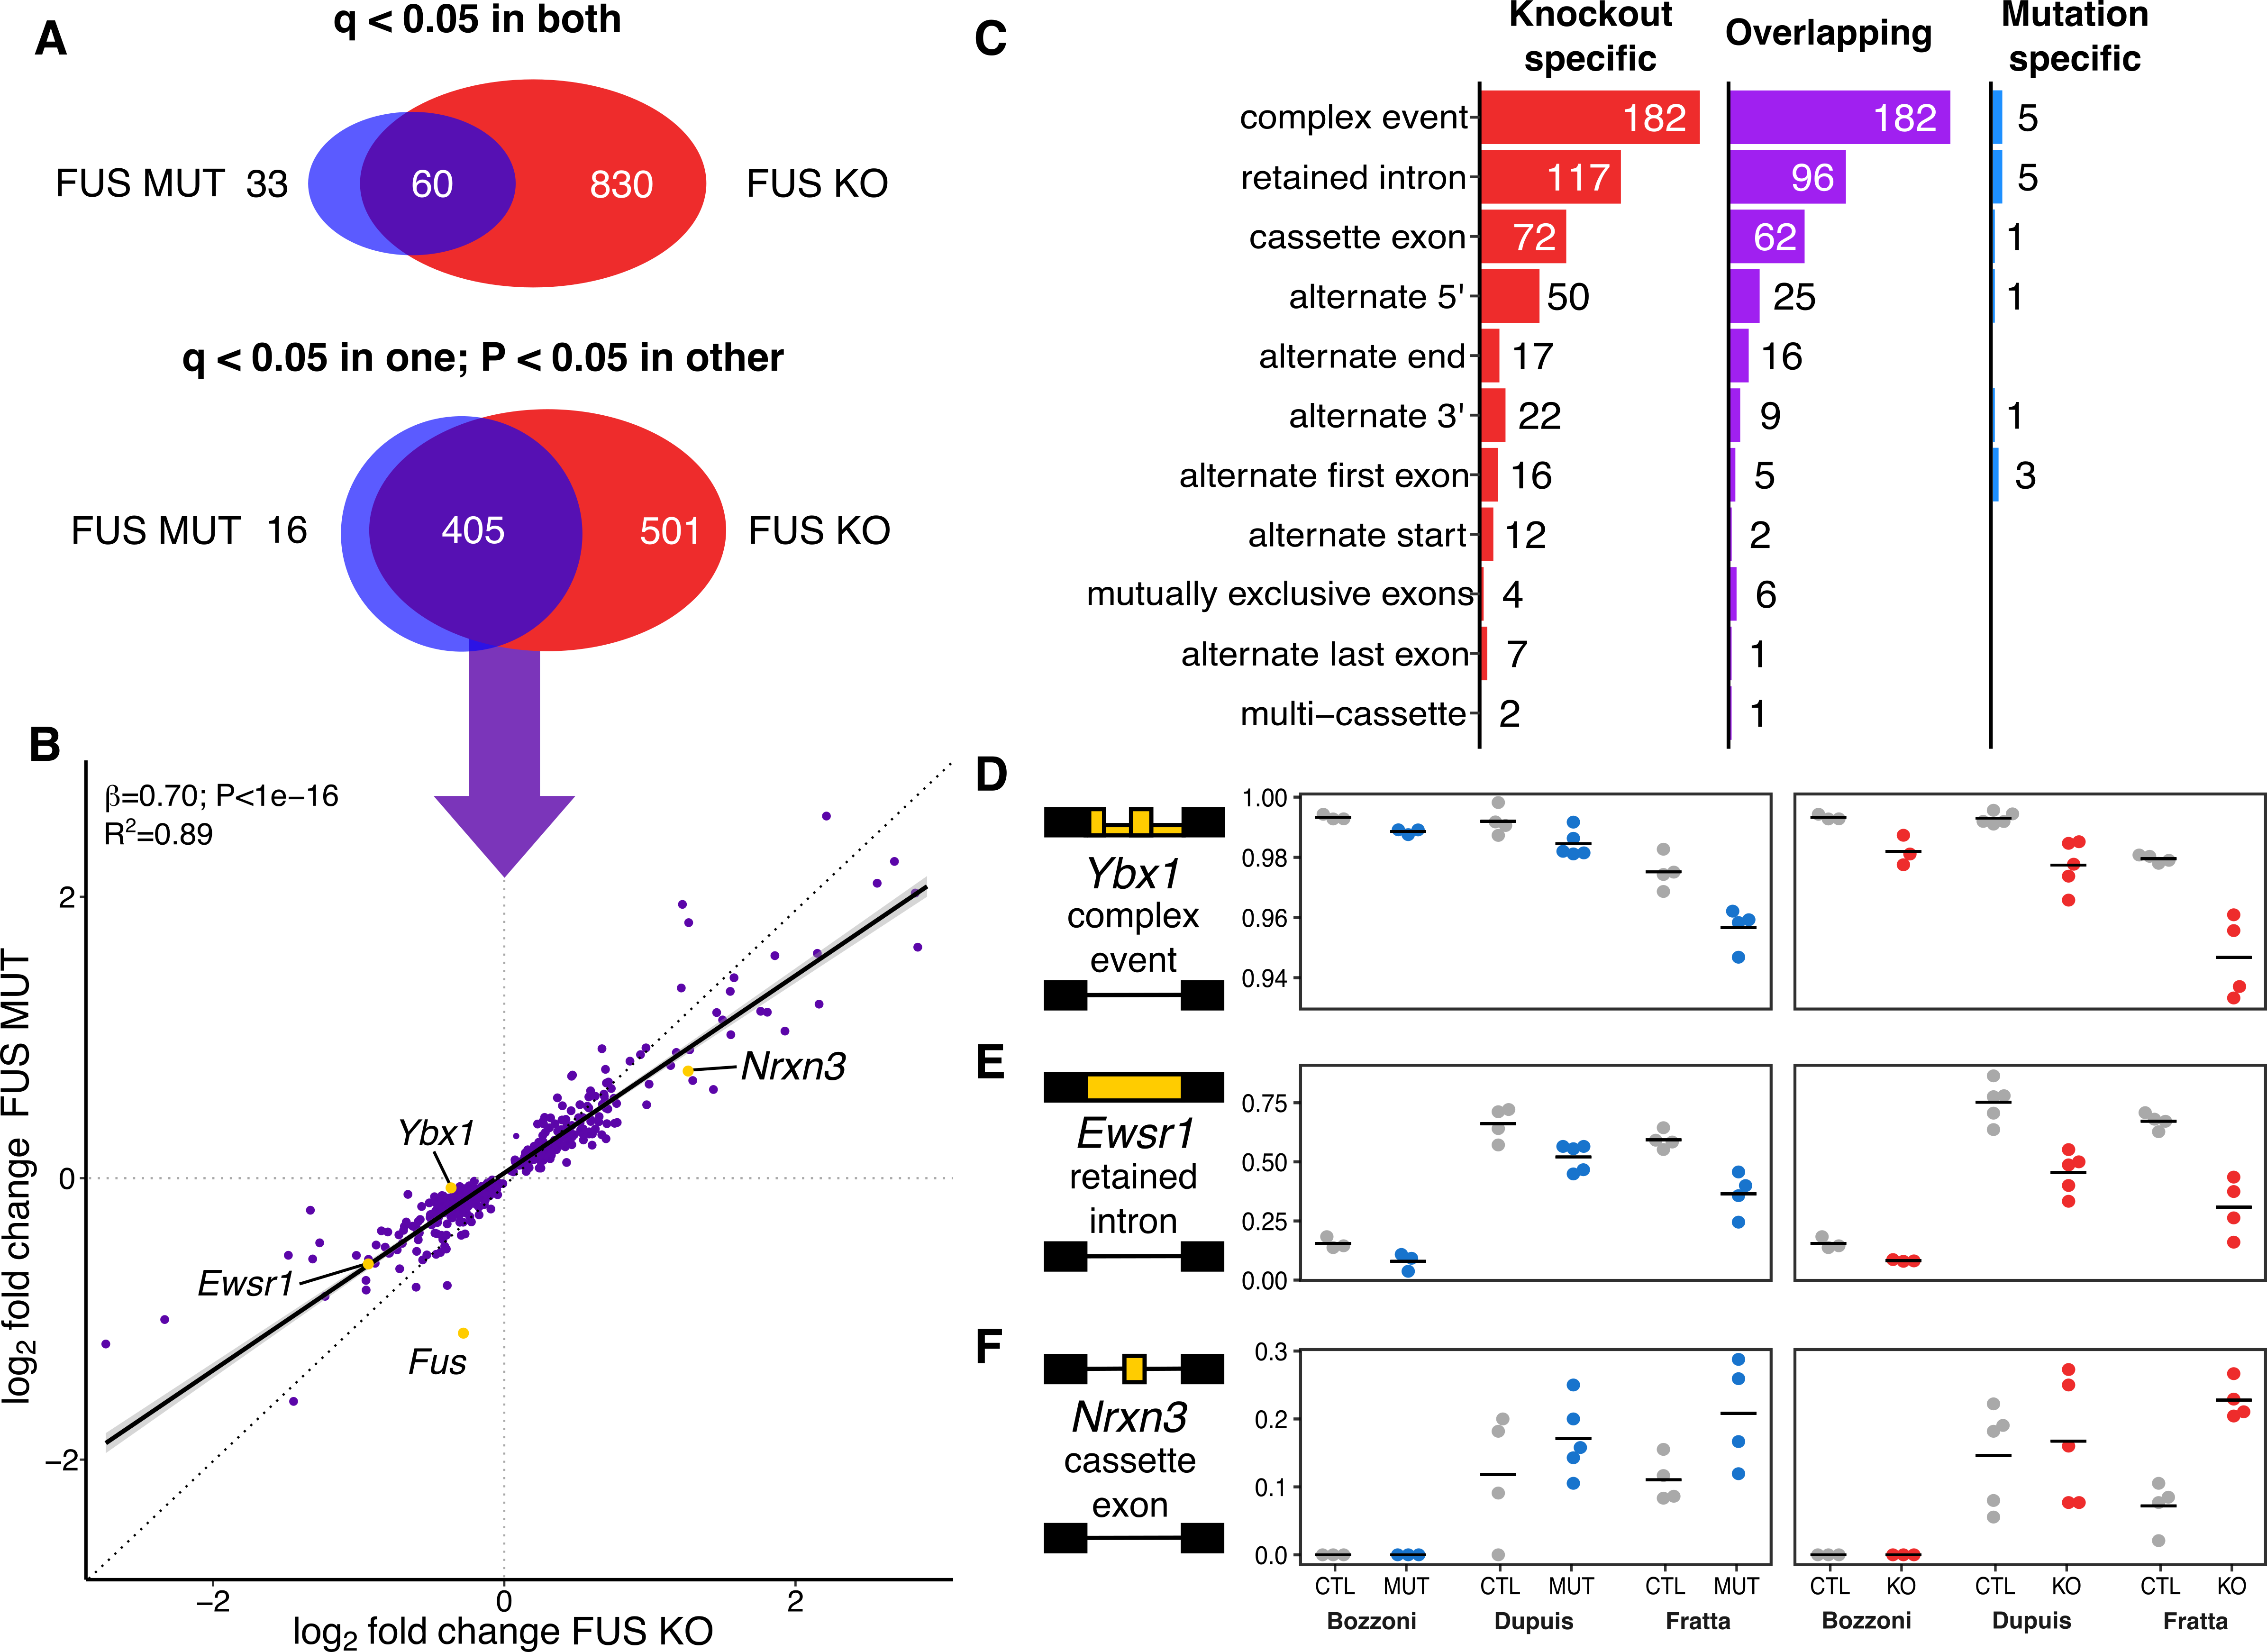
\includegraphics[width=\textwidth]{Figures/06_fus_meta/splicing_multi.png}
	\caption{\textbf{Splicing changes  strongly overlap between KO and MUT joint models}}
	A: Overlapping KO and MUT splicing events results in a significant overlap. The number of mutation specific events drops to just 16 when a more relaxed overlap threshold is used.
	B: Splicing events plotted by their $log_2$ fold change values in the KO and MUT joint models. There is a bias towards larger changes in the KO than MUT ($\beta = 0.7$; .P < 1e-16).
	C: Categories of splicing variant found in each set of events. Complex events are defined as splicing events which are made up of multiple categories.
	D-F: Examples of a cassette exon, retained intron and a complex event in all three datasets. 
	\label{fig:fus_splicing_multi}
\end{figure}

Comparing the strict to the relaxed overlap criteria between the KO and MUT joint models \ref{fig:fus_splicing_multi}, again the relaxed overlap greatly reduces the number of events found to be specific to FUS mutation to just 16, with 405 overlapping events and 501 found to be specific to FUS knockout. 
Plotting the $log_2$ fold changes of the overlapping splicing events, there is a similar trend towards fold changes being stronger in the KO than the MUT joint models ($\beta$ = 0.7, P < 1e-16; F-test; $R^2$ = 0.89). 
There are no overlapping splicing events that change in opposing directions between KO and MUT.

\begin{figure}[h!]
	\centering
	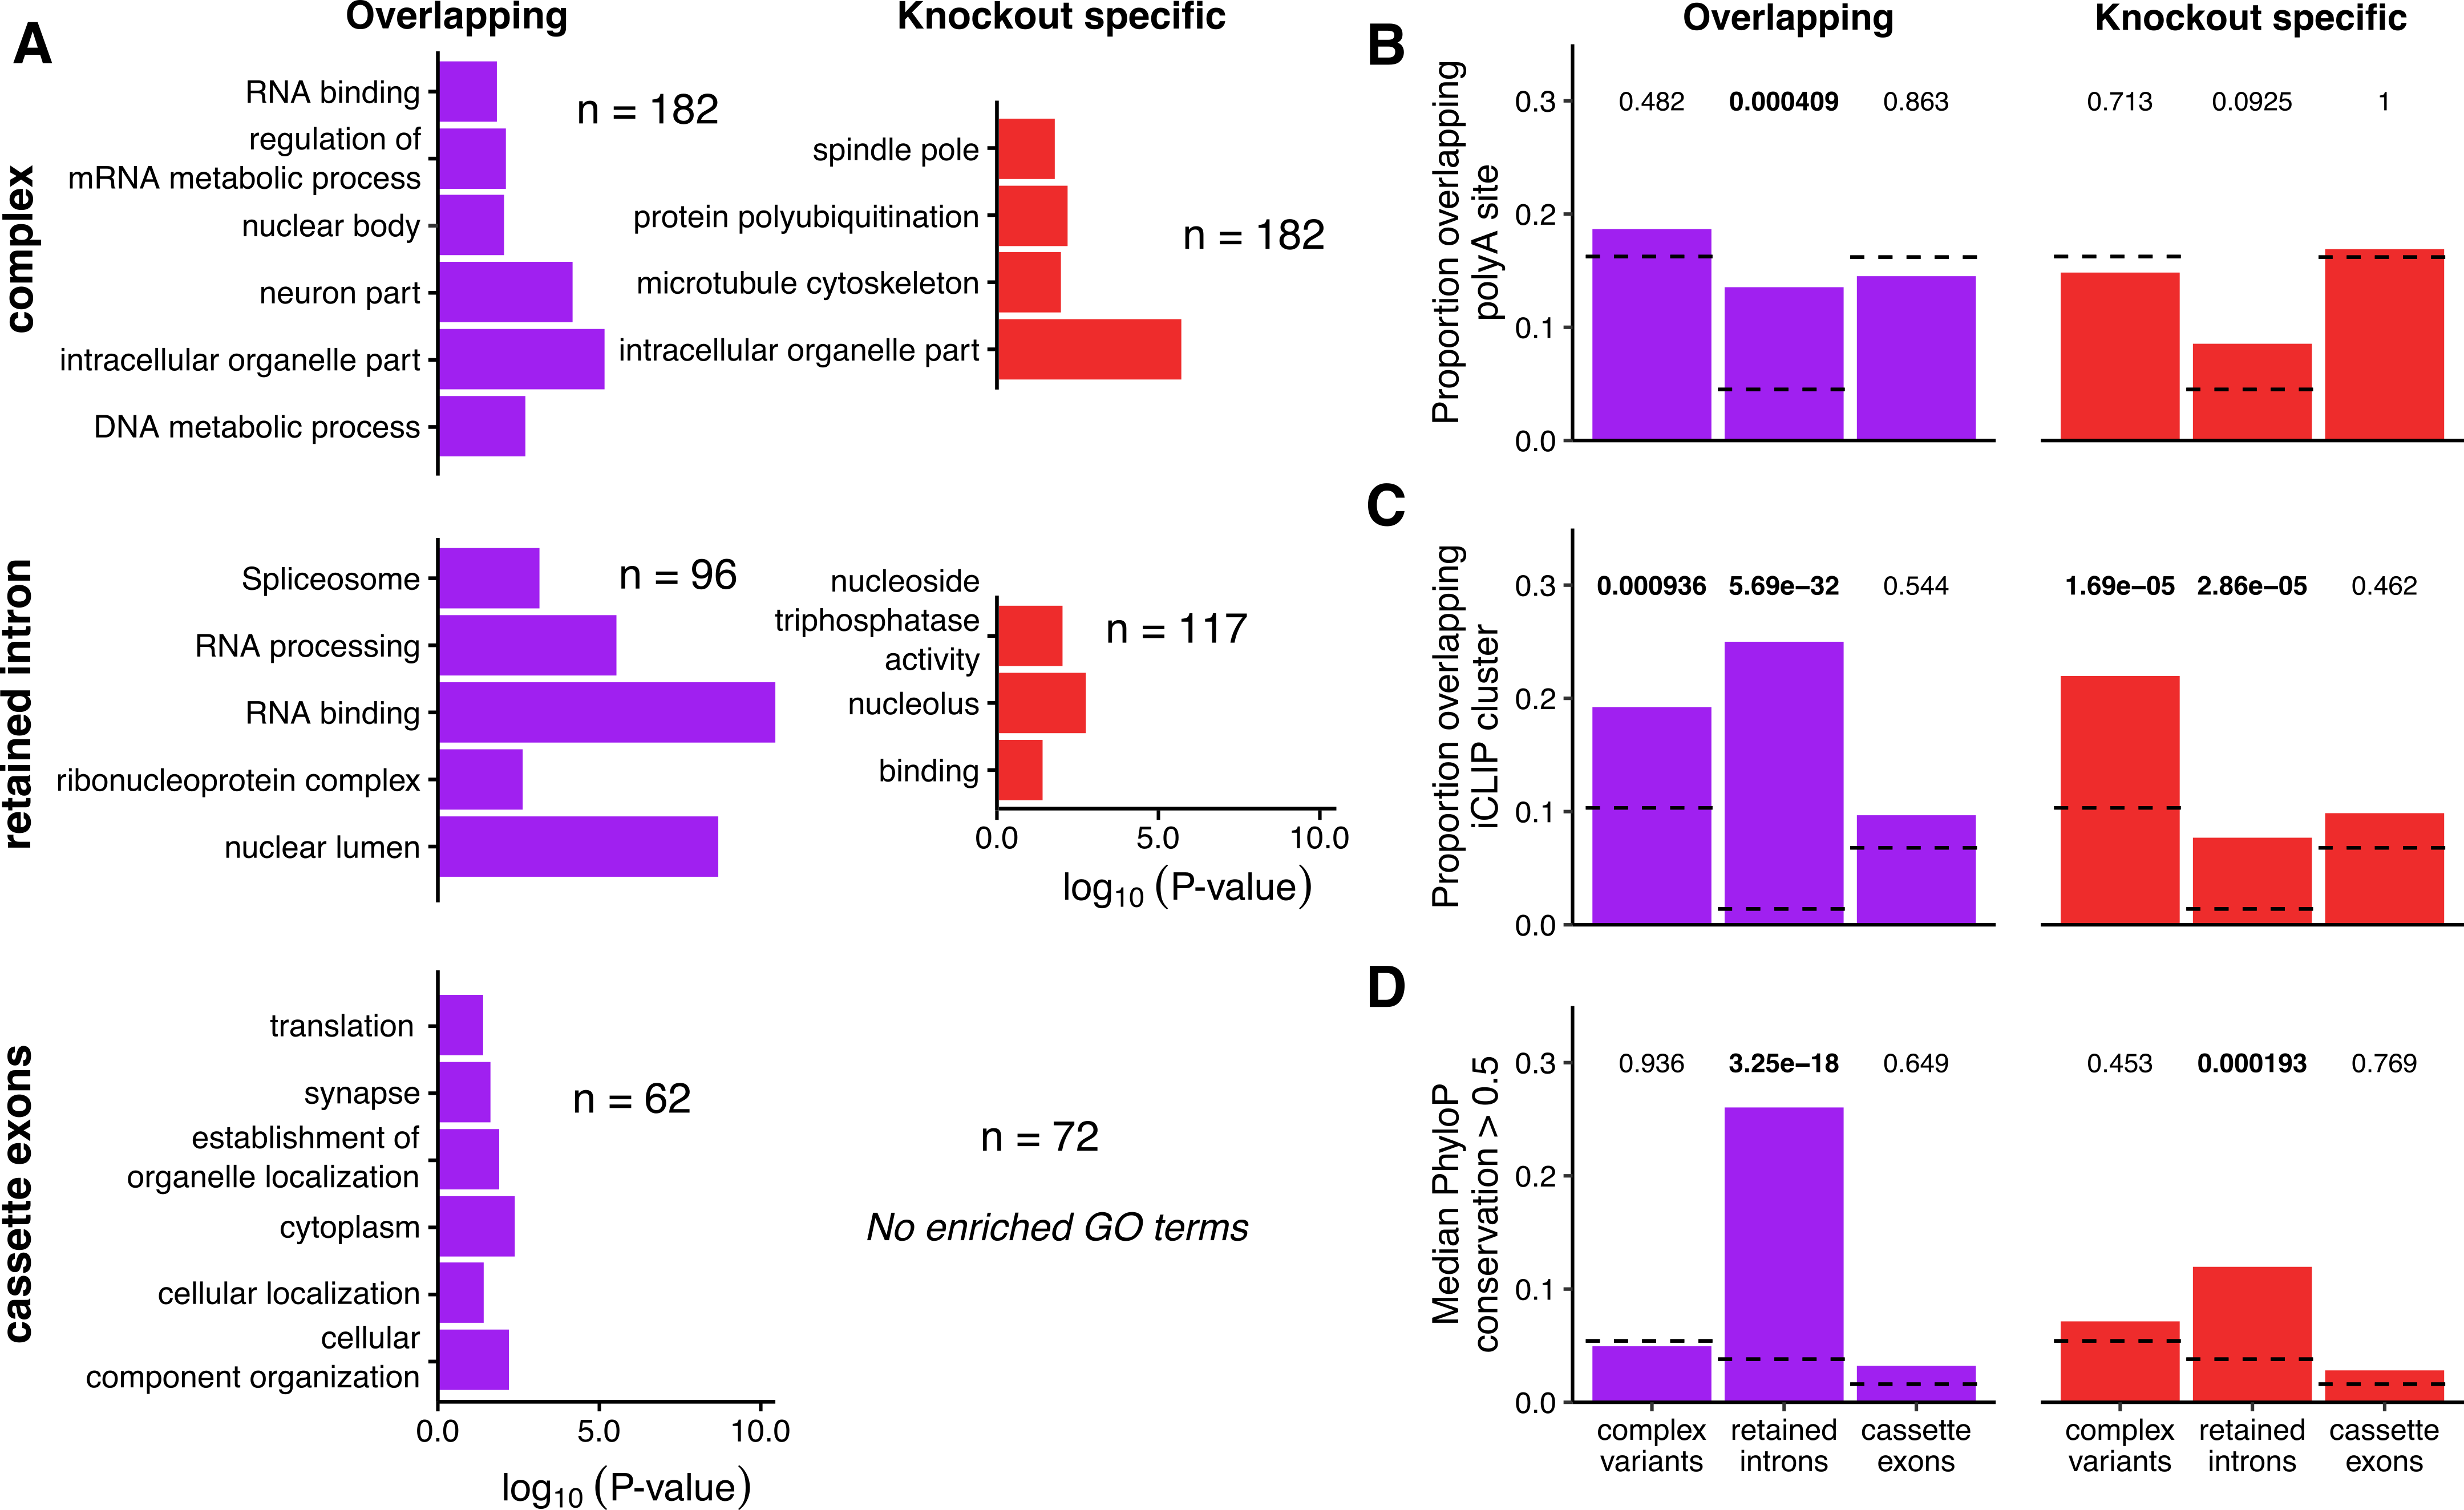
\includegraphics[width=\textwidth]{Figures/06_fus_meta/splicing_go_functions.png}
	\caption{\textbf{Intron retention events are highly conserved and occur in RNA binding proteins} }	
	A: Significantly enriched Gene Ontology terms found in genes split by category and splicing variant type.
	B: The proportion of each type of splicing variant in each category that overlaps a polyadenylation cleavage site.
	C: The proportion of each type of splicing variant in each cateoory that overlaps a FUS iCLIP peak.
	D: The proportion of each type of splicing variant in each category that have a median PhyloP conservation score greater than 0.5.
	\label{fig:fus_splicing_functions}
\end{figure}

The three largest categories of splicing events for the knockout-specific and overlapping events were complex, retained intron and cassette exons. 
I subjected each category to enrichment tests both for gene ontology terms and other genomic features. separating splicing events into complex, retained introns and cassette exons.
There was a clear enrichment in RNA-binding and neuronal GO terms in the overlapping splicing events, with RNA binding terms dominating retained introns and neuronal terms in cassette exons \ref{fig:fus_splicing_functions}. 
Less specific terms appeared in the knockout-specific splicing events.

FUS has been observed to modulate polyadenylation \citep{Masuda2015}.
It is possible that some of the complex and intron retention events are actually differences in polyadenylation site usage.
I compared each set of splicing events with a set of annotated polyadenylation sites \citep{Gruber2016} and compared each set to a random null expectation.
Only overlapping retained introns were enriched for polyadenylation sites (P = 0.004).
To look for evidence of direct regulation by FUS of these splicing events I used the same set of FUS iCLIP clusters from \citep{Rogelj2012}.
Complex events and retained introns were enriched having iCLIP clusters nearby in both overlapping and knockout-specific contexts, with the strongest enrichment seen in overlapping retained introns (P = 5e-32). No enrichment was seen in cassette exons, suggesting that cassette exon splicing changes are not the direct result of a change in FUS binding.
RNA-binding proteins often contain intronic sequences that are very highly conserved \citep{Lareau2007} and these sequences are often used in the regulation of their translation \citep{Ni2007}.
To test whether the splicing events show high sequence conservation, I calculated the median PhyloP score using the 60-way comparison between mouse and other species for each encompassing intron \citep{Pollard2010-fj}.
Sets of events were then tested on the proportion of the set with a median phyloP score > 0.5, where a score of 0 is neutral and 1 is highly conserved.
Only retained introns were shown to be enriched in sequence conservation, and particularly so for those found to be overlapping (P = 3e-18) than in knockout-specific events (P = 0.0002). For cassette exons the two flanking introns are included and so the median conservation score will reflect the conservation of those introns, even when the central cassette exon itself is highly conserved.

Taken together, these results show that nuclear loss of FUS through either knockout or NLS mutation leads to a set of splicing changes concentrated in conserved intron retention events affecting RNA-binding proteins. Cassette exons do not tend to be bound by FUS beyond the null expectation and come from poorly conserved introns.

% overlap splicing and gene expression
As the splicing events are enriched for similar gene ontology terms as the differentially expressed genes, I reasoned that these may affect the same group of genes.
However, only 59 differentially expressed genes are found to contain a splicing event. 
Of those 59, only 12 have FUS iCLIP binding peaks (17\%).. 
Those 12 genes all have either complex or retained intron events and includes the U1 splicing factor \textit{Snrnp70}, the FET protein family members \textit{Ewsr1} and \textit{Taf15}, and \textit{Fus} itself. 
This analysis shows that the role of FUS on gene expression and splicing is largely mutually exclusive.


% TABLE OF SPLICING EVENT COUNTS
\begingroup
\renewcommand{\arraystretch}{1.5} 
\begin{table}[h!]
	%\begin{centerline}
		\begin{tabular}{|r|ccc|ccc|}
			\hline
			%\centering
			& Bozzoni & Dupuis & Fratta & Bozzoni & Dupuis & Fratta\\[-0.3cm]
			& MUT & MUT & MUT & KO & KO & KO\\
			\hline
			Individual hits                & 47 & 1 & 79 & 275 & 54 & 316 \\
			Overlapping joint model & 9 & 0 & 33 & 143 & 31 & 206 \\
			Unique to dataset          & 38 & 1 & 46 & 68????? & 23 & 110 \\
			\hline
			\textbf{Joint model}       & \multicolumn{3}{c|}{93} & \multicolumn{3}{c|}{890} \\
			\hline
			Overlap (strict)              & \multicolumn{2}{c|}{33} & \multicolumn{2}{c|}{\textbf{60}} & \multicolumn{2}{c|}{830} \\
			Overlap (relaxed)           & \multicolumn{2}{c|}{16} & \multicolumn{2}{c|}{\textbf{405} } & \multicolumn{2}{c|}{501} \\
			\hline
		\end{tabular}
	%\end{centerline}
	\caption{Results from separate and joint splicing analysis}
	\label{tab:splicing_results}
\end{table}
\endgroup

\subsection{FUS autoregulation is dependent on intron retention}

\begin{figure}[h!]
	\centering
	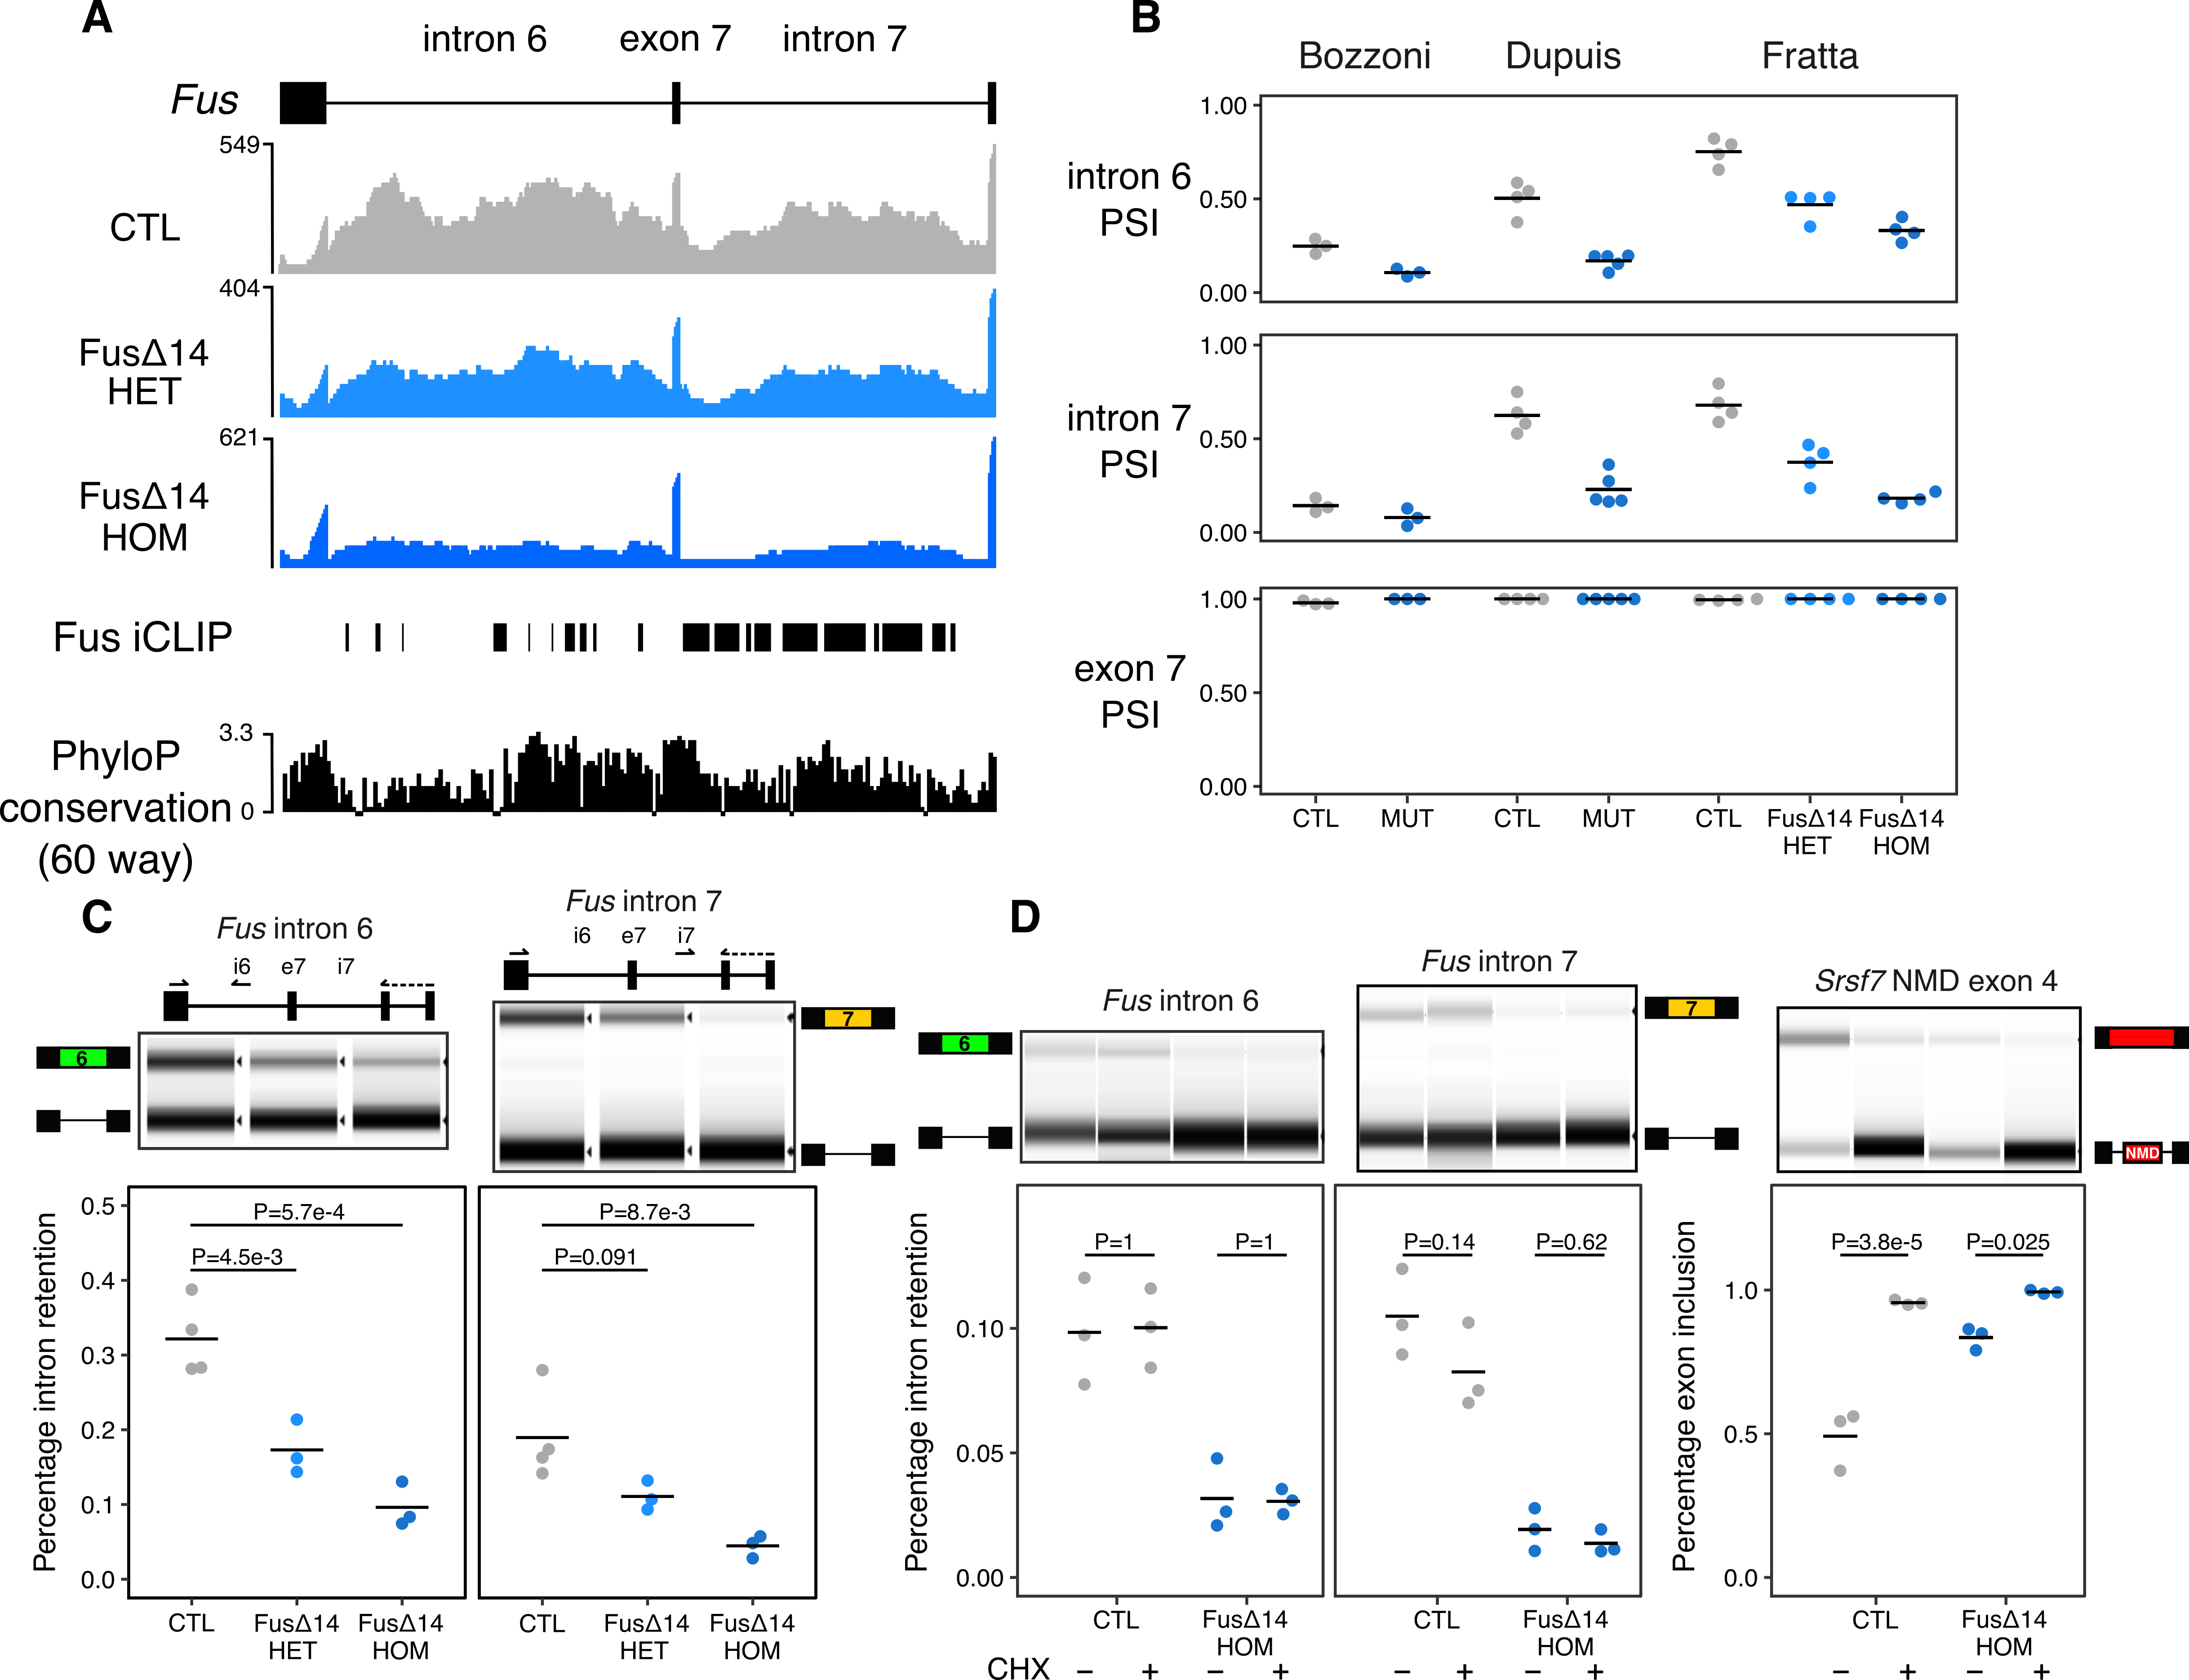
\includegraphics[width=\textwidth]{Figures/06_fus_meta/Fus_autoregulation.png}
	\caption{\textbf{Fus intron retention is an NMD-insensitive autoregulation mechanism } }
		A: FUS introns 6 and 7 are highly conserved and have multiple FUS iCLIP binding peaks. 
		Retention of introns 6 and 7 is decreased with increasing dose of the Fus $\Delta$14 mutation. 
		RNA-seq coverages for example wildtype, FUS $\Delta$14 heterozygous and Fus $\Delta$14 homozygous samples are accompanied by Fus iCLIP and PhyloP conservation (60 way) tracks.
		B: Percentage spliced in (PSI) values of intron 6, intron 7 and exon 7 in the three datasets, including the Fus $\Delta$14 heterozygotes.
		C: RT-PCR validation of the reduction in intron 6 and 7 inclusion with increasing dose of Fus $\Delta$14 mutation. 
		Left panel - \textit{Fus} intron 6 (ANOVA genotype P = 5.1e-4; t-test CTL vs HET P = 4.5e-3; CTL vs HOM P = 5.7e-4)
		Right panel - \textit{Fus} intron 7 (ANOVA genotype P = 8.5e-3; t-test CTL vs HET P = 0.091, CTL vs HOM P = 8.7e-3 )
		D:	Translation blocked with cycloheximide (CHX) to observe whether the intron retention transcript is sensitive to nonsense-mediated decay. 
		Left panel: \textit{Fus} intron 6 retention is not altered with CHX treatment. ANOVA treatment P=0.96; genotype P=1.9e-5; t-test CTL untreated vs CTL treated P=1; HOM untreated vs HOM treated P=1.
		Middle panel: \textit{Fus} intron 7 retention is unchanged by CHX treatment. ANOVA treatment P=0.10; genotype P=3.7e-6; t-test CTL untreated vs CTL treated P=0.14; HOM untreated vs HOM treated P=0.62.
		Right panel - \textit{Srsf7} exon 4, a known NMD target, is increased by CHX treatment. ANOVA treatment P=5.3e-4; genotype P=0.011; t-test CTL untreated vs CTL treated P=3.8e-5; HOM untreated vs HOM treated P=0.025.
		All reported P-values are corrected for multiple testing.
	\label{fig:fus_autoregulation}
\end{figure}


% explain FUS autoregulation
The joint splicing analyses found 5 splicing events in FUS itself, all of which are retained introns. 3 of the 5 are knockout-specific so we assume these are artefacts of partial FUS knockout in the Bozzoni dataset. 
However, The 2 remaining introns (introns 6 and 7) were found to be present in the FUS NLS mutants.
These introns overlap a large number of FUS iCLIP binding peaks.
We reasoned that these events may be an RNA response to reduced nuclear FUS protein.
Many RNA-binding proteins have the ability to bind their own RNA, which creates  a positive feedback loop to tightly control the level of their own translation, a phenomenon known as autoregulation.
When protein levels are high, protein-RNA binding splicing towards the production of an untranslated isoform.
This is commonly through exposing transcripts to nonsense-mediated decay \citep{McGlincy2008-wh}, by including an exon containing a premature stop codon as in HNRNP L and NOVA \citep{Rossbach2009,Dredge2005}, skipping a frame-preserving exon as in PTBP1 \citep{Wollerton2004}, or splicing within the 3'UTR as in TDP-43 \citep{Ayala2011}. 

RNA-protein interaction experiments have revealed a large cluster of FUS binding across introns 6 and 7 of the FUS gene \citep{Lagier-Tourenne2012}, both of which show very high sequence conservation between species.
This region was previously suggested to be the locus of autoregulation due to both an annotated cassette exon event in exon 7 and an a early polyadenylation transcript being present in transcript annotation databases.
Zhou and colleagues first investigated the mechanism of FUS autoregulation by inhibiting nonsense-mediated decay and looking at changes in splicing of exon 7 \cite{Zhou2013}.
Skipping of exon 7 is predicted to cause a frameshift and trigger nonsense-mediated decay. 
The exon-skipping transcript decreased when FUS was overexpressed, suggesting this splicing event to be the autoregulatory mechanism.
However this mechanism does not explain the high sequence conservation of the diffuse FUS binding pattern across introns 6 and 7 (Figure \ref{fig:fus_autoregulation}A).
When examining our RNA-sequencing coverage of the FUS gene as well as that of Bozzoni and Dupuis, I could not observe any changes in the inclusion of exon 7 in any sample.
However I could observe a strong retention of both introns 6 and 7 decreases in the presence of FUS NLS mutations. 
This effect can be seen in all three datasets (Figure \ref{fig:fus_autoregulation}B), despite the baseline level of retention in wildtype cells being highly variable. 
We generated RNA sequencing data from mice heterozygous for the $\Delta$14 NLS mutation. Retention of introns 6 and 7 clearly decreases with dose of the mutation.

We designed an RT-PCR assay to validate the intron retention changes with a three primer method that could amplify spliced a FUS exon 6-7-8-9 transcript with a second band for either exon 6-intron 6 or intron 7-exon8. 
Intron retention decreased in a mutation dose-dependent manner (intron 6 P = 5.7e-4; intron 7 P = 8.7e-4; ANOVA; Figure \ref{fig:fus_autoregulation}C).
We failed to detect a band corresponding to the skipping of exon 7 in any sample. 

Retaining two introns would be expected to cause nonsense mediated decay (NMD) through premature stop codons, which are abundant in both intron 6 and 7. 
This has been proposed as the main degradation pathway for intron retention transcripts \citep{Wong2013}, although the RNA surveillance pathway has also been implicated \citep{Yap2013}. 
To test whether the intron retention FUS transcript undergoes nonsense-mediated decay we reran the RT-PCR experiments after treating mouse fibroblasts with cycloheximide for 6 hours to inhibit translation, as well as NMD.  
No effect on intron retention by cycloheximide treatment was seen in either wildtype of FUS $\Delta$14 homozygous fibroblasts (Figure \ref{fig:fus_autoregulation}D).
Despite this, NMD was definitely inhibited as the inclusion of a known poison exon in \textit{Srsf7} \citep{Edwards2016} was increased in both genotypes. 

These experiments suggest that depleting nuclear FUS protein downregulates the production of an intron retention transcript insensitive to nonsense-mediated decay. 




%Yap2013 - intron retention in neurons of terminal 3' introns detains neuronal-specific transcripts in the nucleus which are eventually degraded not by NMD but by RNA surveillance proteins. and then switch to splicing out and cytoplasmic transport when Ptbp1 levels change

% negative feedback mechanism
% protein homeostasis
% protein binds own mRNA
% changes in protein levels alters the splicing of the mRNA from a productive isoform to an isoform susceptible to nonsense-mediated decay, by skipping a frame-conserving exon, or by introducing a poison exon.
% iCLIP experiments have revealed that Fus binds a large section of its own mRNA spanning ~ 3500bp comprising intron 6, exon 7 and intron 7. 
% Both introns show very high conservation between species, suggesting an important regulatory role for the introns.
% \cite{Zhou2013} and colleagues used RT-PCR to show that changes in FUS protein levels alters the inclusion of exon 7 and the exon 7-skipped transcript is sensitive to nonsense-mediated decay.
% Inspecting the RNA-seq traces from our data as well as Dupuis and Bozzoni, we see no evidence for any change in exon 7 inclusion in the presence of NLS mutated FUS.
% Instead we see a clear reduction in the retention of introns 6 and 7.
% Using RNA-seq data from the heterozygous FUS $\Delta$14 mice it is clear that the reduction in intron retention is dependent on the mutation dosage.

% To validate the intron retention changes I developed an RT-PCR assay with primers targeting exon 6 and exons 8/9 to selectively amplify spliced FUS mRNA and an additional third primer targetting either intron 6 or intron 7. This three primer PCR amplifies bands corresponding to intron 6 and 7 retention and splicing. Our primers did not amplify a band corresponding to exon 7 skipping. 
% With increasing dosage of the FUS $\Delta$14 mutation the proportion of intron retention reduces for both intron 6 and intron 7 (Figure \ref{fig:fus_autoregulation}C).



\clearpage
\section{Discussion}

% Reiterate what I've done and seen
This study is the largest transcriptome-wide assessment of FUS function to date.
By combining three separate datasets of FUS knockdown and NLS mutation I have been able to discover a large repertoire of differentially expressed genes and differential splicing events.
Comparing the two conditions demonstrates that NLS mutations predominantly act to reduce nuclear FUS as the majority of expression and splicing changes overlap and have the same direction of effect.
This leaves only a small number of NLS mutation-specific gene expression changes.
By studying the effects of NLS mutation on the whole FUS gene I have discovered a novel intron retention transcript that could be the major mechanism by which FUS regulates its own translation.

% Largest transcriptome-wide study of FUS function to date
% Discovered a large number of differentially expressed genes and differential splicing events
% Discovered a novel mechanism for FUS autoregulation via intron retention.

%% Joint modelling

% Importance of replication
% RNA is inherently noisy
% Joint modelling provides clarity

% Joint models boost power but they reward conformity between datasets
% There may be important biological differences, such as subtle cell type or developmental differences that account for different genes and splicing events ocurring in different datasets

% Between sample variance clearly important to detecting RNA changes
% Unexplained why such a difference
% Any evidence of a polyA / total RNA effect on variance?


The joint modelling approach has allowed me to combine three different RNA sequencing datasets from different cell types and produce a consensus set of RNA phenotypes.
Due to the stochastic nature of RNA, this data is inherently noisy. 
By combining repeated observations  under the same genetic conditions we can better understand the true effect of these changes.
Joint models boost detection power but they also reward conformity. 
I can not discount the possibility that each dataset has specific changes due to cell-type or the specific NLS mutations that are being removed by the model.
With increased power, I can now detect effect sizes of expression and splicing that are very small and so the biological relevance of these small changes is harder to investigate.
These changes are less likely to be the result of direct FUS interaction and may through multiple effectors.
As a disease-associated protein, FUS has been intensely studied and the number of putative roles it has within the cell is astronomically large.  Therefore, assigning any one mechanism to a particular change is exceedingly difficult.
%% Gene expression
% We find the largest set of gene expression changes associated with FUS depletion.
% Knockout and NLS mutation have a strong overlap that is biased towards the knockout
% This makes biological sense as NLS mutations don't completely ablate nuclear import
% 99% of genes go in the same direction but 7 genes are upregulated in the FUS mutant
% P values are unconvincing but 3/7 have FUS binding so could be real, worth following up

Comparing the two joint differential gene expression models with a relaxed significance threshold demonstrated that the majority of gene expression changes were shared between knockout and NLS mutation.
On top of that, the direction of change was identical for 99\% of overlapping genes with a bias towards stronger changes in the knockout. 
As NLS mutations do not completely ablate FUS nuclear import this is unsurprising. 
In aggregrate there are some clear trends revealed by gene ontology enrichment. 
% neuronal gene loss
There is a widespread downregulation of neuronal and synaptic specific genes in FUS nuclear depletion. 
This could be due to defects in RNA transport as FUS has been found in RNA transport granules \citep{Kanai2004, Fujii2005}.
% splicing factor upregulation
Conversely, RNA binding genes were upregulated in both conditions. 
FUS is known to interact on a protein-protein level with multiple splicing factors \citep{Yang1998,Meissner2003, Groen2013} and particularly members of the U1 snRNP complex \citep{Sun2015a, Yu2015} and FUS binds a number of these factors at the RNA level \citep{Nakaya2013}.
% Xlr genes
I managed to replicate the finding of upregulation of the X-linked lymphocyte receptor (Xlr) cluster of genes, first seen in adult FUS knockout mice \citep{Kino2015}, suggesting that FUS loss causes chronic dysregulation of these genes. 
As Xlr gene over-expression can alter dendritic spine growth \cite{Cubelos2010}, the mechanism of how FUS loss leads to their upregulation is intriguing. 
No FUS iCLIP peaks were observed overlapping any Xlr gene, discounting post-transcriptional regulation.


% Splicing
Overlapping the joint splicing models demonstrated that almost all splicing changes in NLS mutations could be observed in knockouts.
I did not observe a convincing set of mutation-specific splicing changes which is unsurprising as splicing is a nuclear function. 
The overlap between knockdown and expression has been seen in cells where overexpression of NLS mutant FUS cannot rescue splicing changes in FUS knockdown cells \citep{Sun2015a}.
FUS known to interact with Pol II, U1 and the survival of motor neuron (SMN) protein \citep{Schwartz2012, Yu2015} so disturbance of all of these factors could be confounding splicing changes. 
The splicing profiles of FUS NLS mutations overlaps with SMN haploinsufficency \citep{Mirra2017}.
I observed double the number of 5' splice site changes than 3' splice site changes. This could be due to the shorter length of the consensus 5' splice site sequence compared to the 3' making cryptic splice sites more likely by chance, but it may hint at a consequence of the interaction between FUS and the U1 snRNP.
The dominance of retained introns and complex events where multiple splice sites are altered simultaneously also points to large scale changes in the spliceosome as opposed to alterations in specific RNA-binding proteins.
Retained introns and complex events are enriched in FUS iCLIP binding and are more likely to affect splicing factors than the cassette exons I observed. 
This suggests a more subtle role for FUS in splicing than simply altering alternate exons which were the focus on previous studies on FUS and splicing.
The large number of cpmplex events seen in the joint splicing models is probably a result of the juction-centric method I used, as well as analysing all the data jointly. 
An isoform-centric approach where reads are assigned to specific transcripts \citep{Trapnell2010,Bray2015} perhaps would more sensitively tease out the different changes that are happening in complex introns.

The high sequence conservation seen in retained introns suggests a regulatory role for these splicing events, despite the unexpectedly low overlap between splicing changes and differentially expressed genes.
The exception to this is the U1 splicing factor \textit{Snrnp70}, whose highly conserved intron retention transcript has previously been shown to increase in FUS knockdown, leading to increased degradation of \textit{Snrnp70} mRNA through nonsense-mediated decay \citep{Nakaya2013}.
The other FET family members \textit{Taf15} and \textit{Ewsr1} are both upregulated in both FUS conditions and both contain conserved intron retention events that are more frequently skipped in FUS depletion.
For \textit{Taf15}, its upregulation in response to FUS loss is probably a redundancy mechanism due to shared RNA motifs and target genes \citep{Kapeli2016,Ibrahim2013}. 
The splicing changes I identify in both \textit{Taf15} and \textit{Ewsr1} suggest a mechanism for how its expression is increased when nuclear FUS is depleted.
A previous study on RNA stability in FUS knockdown did not find \textit{Taf15} to be changed  \citep{Colombrita2012} but this requires reevaluation in light of my new splicing data.

By studying our RNA-seq data in all three NLS mutant datasets I observed a novel intron retention isoform whose retention inversely correlates with the dose of NLS mutation. 
Although cassette exon skipping of exon 7 was previously suggested to be the splicing event of FUS autoregulation, our data suggests that intron retention is more likely.
Neither our RNA-seq or our RT-PCR observed exon 7 skipping in the presense of NLS mutation. 
This could simply be due to exon 7 skipping being present but at much lower level than intron retention changes. 
Zhou and colleagues would not have detected intron retention changes due to the length of the retention transcript exceeding the amplication length for PCR. 
Our three-primer approach robustly demonstrated the changes in retention occur in both introns 6 and 7 but they cannot conclusively prove simulatanous retention of both introns.
This would require a long-read sequencing technique.
Our cycloheximide experiments suggests that the FUS intron retention transcript is insensitive to nonsense-mediated decay. 
Further experiments are needed to validate this transcript in human cells and to test whether the transcript is instead detained in the nucleus, a regulatory pathway proposed for intron retention transcripts to prevent translation \cite{Boutz2015}.

% ALS biology implications
This study pulls together multiple experiments to better understand and catalogue changes in gene expression and RNA splicing in response to FUS nuclear depletion through either knockout or NLS mutation.
My work suggests that these changes are largely shared due to the extreme overlap and concordance of direction of gene expression and splicing.
It does not conclusively link any of these alterations to motor neuron toxicity and degeneration, which is only seen in NLS mutant embryos and not in FUS knockouts \citep{Scekic-zahirovic2016}.
It is unclear whether toxicity can be blamed on the 186 mutation-specific genes due to the sharing of gene ontology categories with the overlapping set (RNA processing and synaptic genes). 

What is of more relevance to understanding the role of FUS in disease is my discovery of potentially the major autoregulatory mechanism for FUS in the doubly retained intron retention transcript.
Autoregulation acts to maintain protein homeostasis but NLS mutations interfere with this mechanism. 
When FUS nuclear import is ablated by mutation there is no way for FUS protein to turn off its own translation, leading to ever-more cytoplasmic FUS.
High concentrations of cytoplasmic FUS increase the likelihood for aggregation which NLS mutant FUS is more prone too. This is presumably due to the recent finding that Transportin binding the NLS acts to solubilise FUS aggregates \citep{Guo2018,Yoshizawa2018,Hofweber2018}.
FUS ALS patients only ever have one copy of the NLS mutant allele so nuclear depletion 


% We see more 5' changes than 3', implicating U1 impairment
% How many of the intron retention changes are due to U1-sensitivity? Are retained introns more sensitive to spliceosomal changes?

% No convincing splicing changes found to be mutation specific
% not surprising as this should be a nuclear function of FUS

% Retained introns are enriched for RNA binding function and FUS binding
% Previously seen for Snrnp70 - U1 factor
% This makes sense as FUS can interact with the whole U1 snRNP
% We have extended this to a larger group of proteins

% Cassette exons are not, this is surprising
% Boris found enrichment of FUS peaks within 200bp  of cassette exons whereas we took the entire intron and found no enrichment. Targeted appraoch is probably better.
% FUS's role in alternative exon splicing perhaps overstated

% Retained introns in RNA binding proteins suggests NMD mechanisms
% FUS is part of network of splicing factors that all cross-regulate
% Not surprising that mislocalisation of FUS triggers changes in other factors
% Taf15 and Ewrs1 obvious candidates to replace FUS, redundancy in system
% Ewrs1 retained intron suggests similar mechanism to FUS, perhaps autoregulatory transcript here too? Should investigate

In the case of FET family member \textit{Taf15}, 

% Complex events inherently difficult to interpret
% Here an isoform-level approach would be more effective
% Caveat is when one is interested in novel isoforms, as are important in TDP biology (cite my papers)

% theme - FUS alters splicing and gene expression of genes coding for proteins that FUS is known to interact with - U1 snRNP, hnRNPs, FET proteins, YBX1 \citep{Groen2013}.


%% Autoregulation 
% We have identified a new mechanism for FUS autoregulation
% Is it prematurely polyadenylated?
% RT-PCR primers are targeting isoform with exon 9 included which should be downstream of any premature polyadenylation site.

% why don't we see the Zhou exon 7?
%% No evidence from RNA-seq so skipping transcript may just be very lowly expressed.
% They wouldn't pick up intron retention due to being too long to amplify by RT-PCR.
% Our data suggests that FUS intron retention changes FUS protein levels through a change in mRNA localisation rather than nonsense-mediated decay
% Cite detained introns paper, Pimental paper.


% Implications for ALS biology

% FUS gain of function may take a long time to appear, all data is embryonic
% All models are homozygous, does not reflect ALS patient biology
